%%%%%%%%%%%%%%%%%%%%%%%%%%%%%%%%%%%%%%%%%%%%%%%%%%%%%%
% A Beamer template for University of Wollongong     %
% Based on THU beamer theme                          %
% Author: Qiuyu Lu                                   %
% Date: July 2024                                    %
% LPPL Licensed.                                     %
%%%%%%%%%%%%%%%%%%%%%%%%%%%%%%%%%%%%%%%%%%%%%%%%%%%%%%
% Customized for Sharif University of Technology     %
%%%%%%%%%%%%%%%%%%%%%%%%%%%%%%%%%%%%%%%%%%%%%%%%%%%%%%

\documentclass[serif, aspectratio=169]{beamer}
%\documentclass[serif]{beamer}  % for 4:3 ratio
\usepackage[T1]{fontenc} 
\usepackage{fourier} % see "http://faq.ktug.org/wiki/uploads/MathFonts.pdf" for other options
\usepackage{hyperref}
\usepackage[absolute,overlay]{textpos}
\usepackage{latexsym,amsmath,xcolor,multicol,booktabs,calligra}
\usepackage{graphicx, pstricks, listings, stackengine, caption, subcaption}
\usepackage{lipsum}

\author{Ali Sharifi-Zarchi}
\title{Machine Learning (CE 40477)}
\subtitle{Fall 2024}
\institute{
    CE Department \\
    Sharif University of Technology
}
%\date{\small \today}
% \usepackage{UoWstyle}
\usepackage{SUTstyle}

% defs
\def\cmd#1{\texttt{\color{red}\footnotesize $\backslash$#1}}
\def\env#1{\texttt{\color{blue}\footnotesize #1}}
\definecolor{deepblue}{rgb}{0,0,0.5}
\definecolor{deepred}{RGB}{153,0,0}
\definecolor{deepgreen}{rgb}{0,0.5,0}
\definecolor{halfgray}{gray}{0.55}

\lstset{
    basicstyle=\ttfamily\small,
    keywordstyle=\bfseries\color{deepblue},
    emphstyle=\ttfamily\color{deepred},    % Custom highlighting style
    stringstyle=\color{deepgreen},
    numbers=left,
    numberstyle=\small\color{halfgray},
    rulesepcolor=\color{red!20!green!20!blue!20},
    frame=shadowbox,
}


\begin{document}

\begin{frame}
    \titlepage
    \vspace*{-0.6cm}
    \begin{figure}[htpb]
        \begin{center}
            
\includegraphics[keepaspectratio, scale=0.25]{pic/sharif-main-logo}
        \end{center}
    \end{figure}
\end{frame}

\begin{frame}    
\tableofcontents[sectionstyle=show,
subsectionstyle=show/shaded/hide,
subsubsectionstyle=show/shaded/hide]
\end{frame}

\section{CNNs in Vision}

\begin{frame}{CNNs are everywhere!}

	\begin{textblock*}{5cm}(7.7cm,1.6cm) % {block width} (coords)
			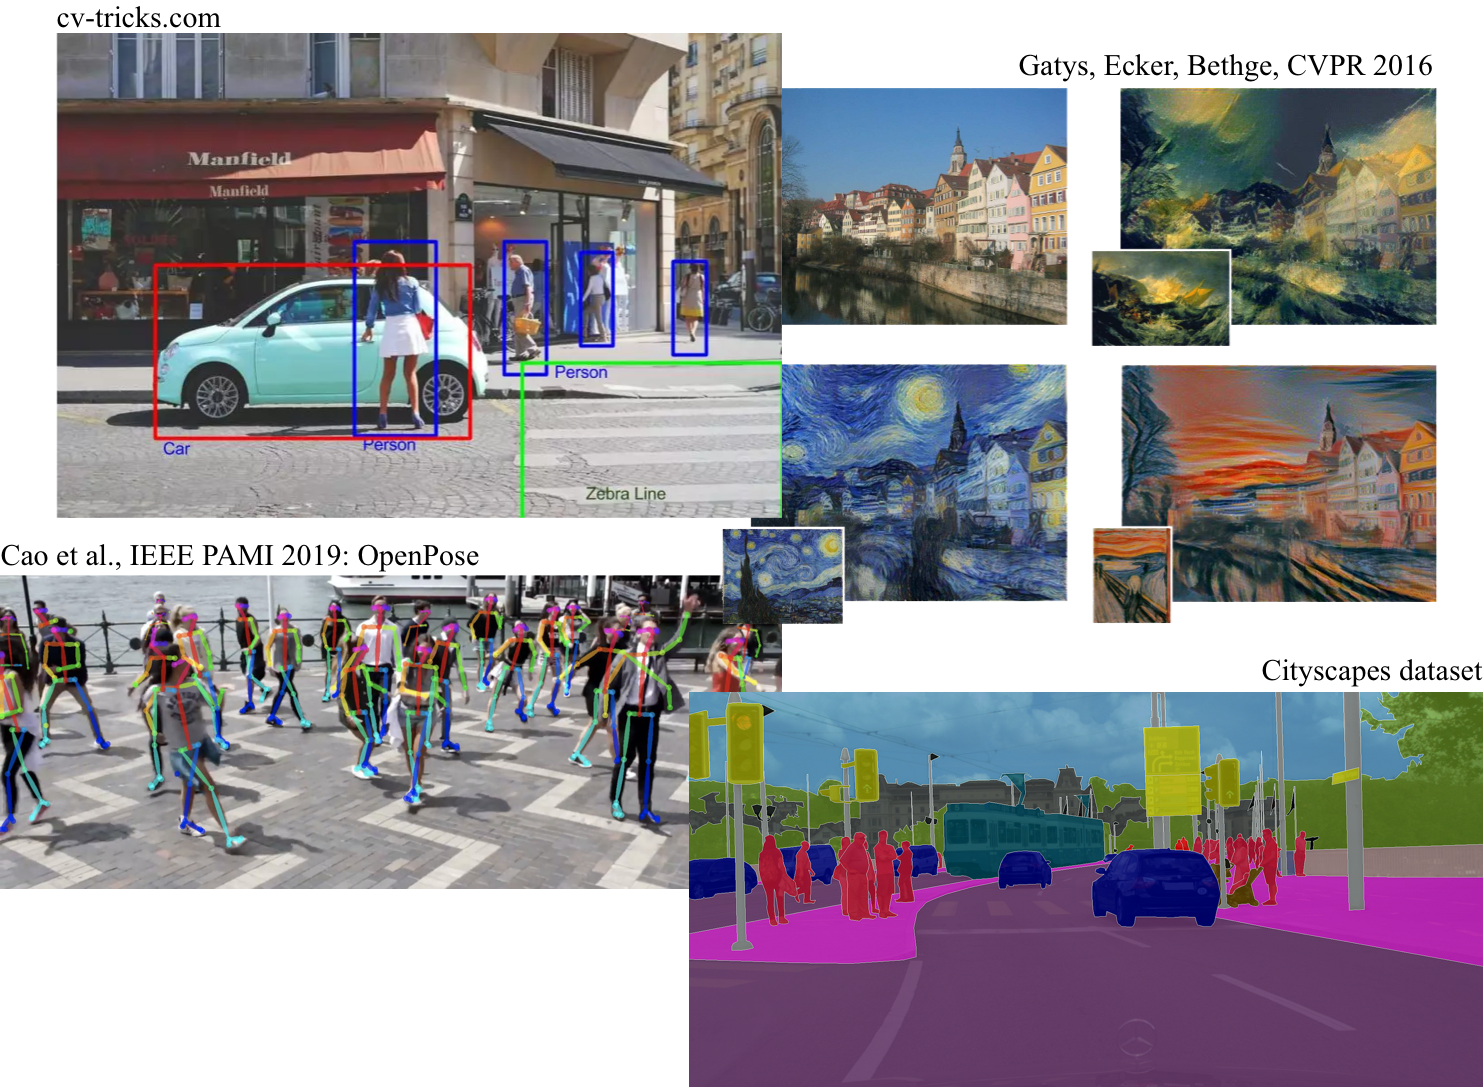
\includegraphics[keepaspectratio, width=8cm]{pic/CNNs}
	\end{textblock*}
	
	\begin{itemize}
		\item The success of deep learning for \newline image recognition has been driven \newline by two key factors:
		\begin{itemize}
			\item Large-scale CNNs
			\item Transfer learning
		\end{itemize}
	\end{itemize}
\end{frame}

\begin{frame}{ImageNet Large-Scale Visual Recognition Challenge (ILSVRC)}
	2009:
	\begin{textblock*}{5cm}(1.9cm,1.44cm) % {block width} (coords)
		
\includegraphics[keepaspectratio, scale=0.2]{pic/imagenet_logo}
	\end{textblock*}
	\begin{itemize}
		\item Dataset and benchmark on image classification
		\item 1 million images with ground truth class labels for training (hand-annotated) 1000 object categories
	\end{itemize}
	\begin{figure}[htpb]
		\begin{center}
			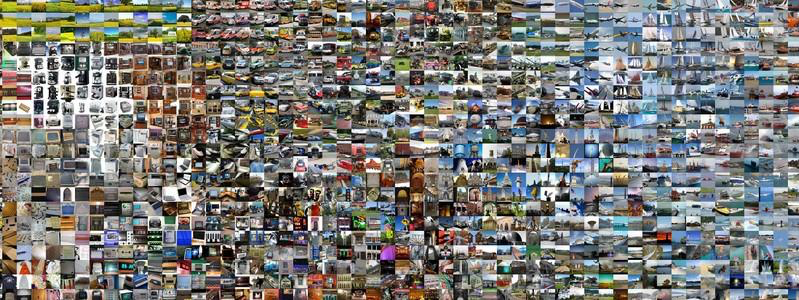
\includegraphics[keepaspectratio, scale=0.35]{pic/imagenet_images}
			\caption*{\scriptsize Deng et al., CVPR 2009}
		\end{center}
	\end{figure}
\end{frame}

\begin{frame}{CNNs are old. Why did it work eventually?}
	\begin{figure}[htpb]
		\begin{center}
			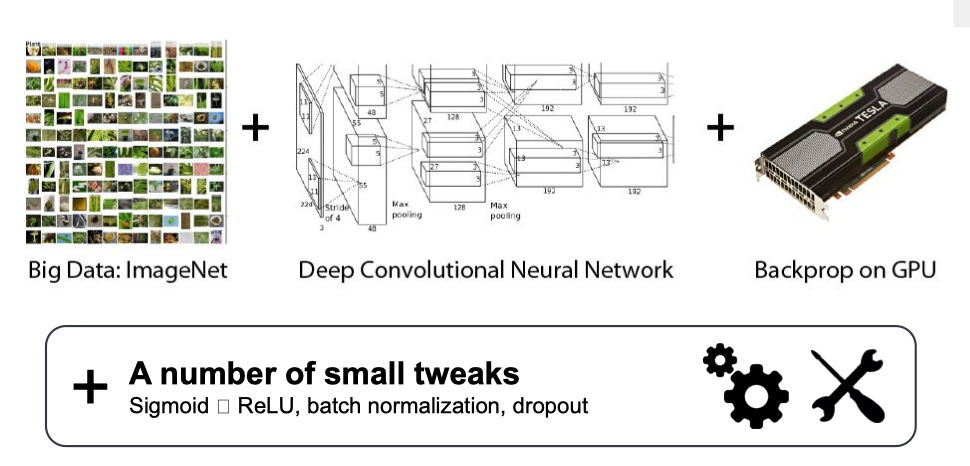
\includegraphics[keepaspectratio, scale=0.37]{pic/gpu}
			\caption*{\scriptsize \href{http://www.andreykurenkov.com/writing/ai/a-brief-history-of-neural-nets-and-deep-learning-part-4}{\color{blue}Image Source}}
		\end{center}
	\end{figure}
\end{frame}

\section{AlexNet}
\begin{frame}{ImageNet Large-Scale Visual Recognition Challenge (ILSVRC)}
	\begin{itemize}
		\item Reduced the error rate by 10 \%
	\end{itemize}
	\begin{figure}[htpb]
		\begin{center}
			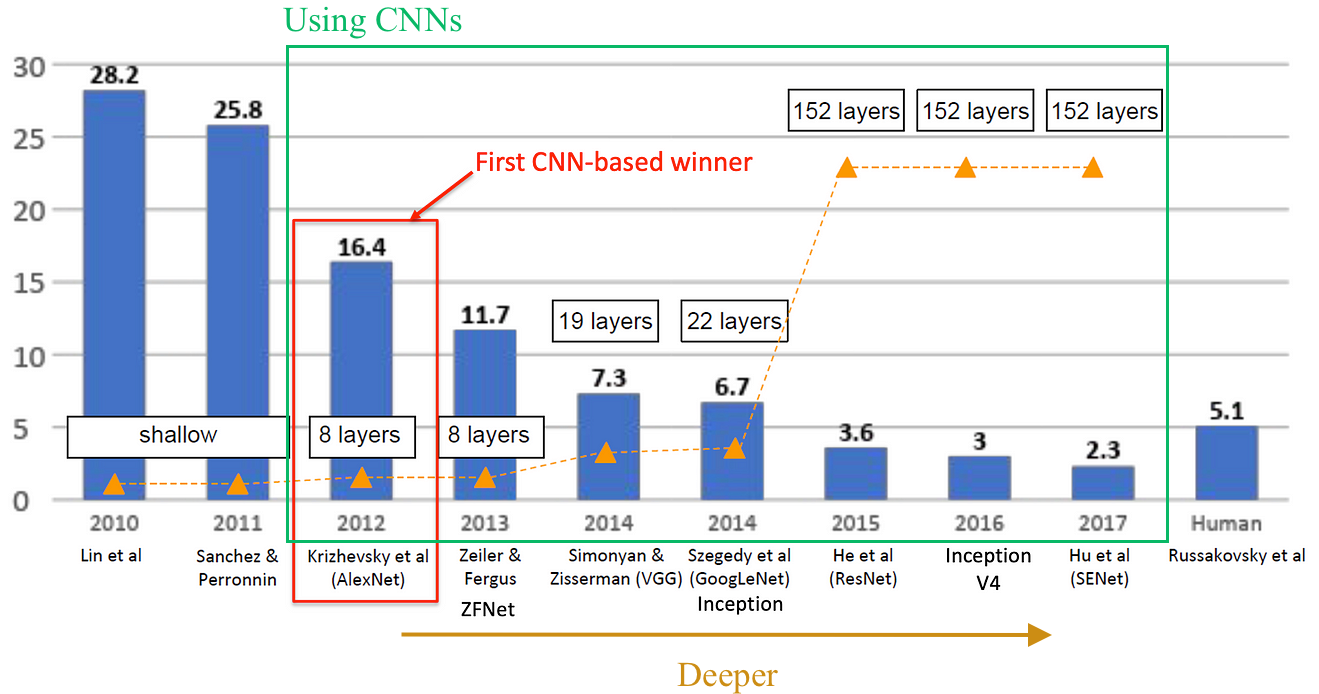
\includegraphics[keepaspectratio, scale=0.25]{pic/imagenet}
		\end{center}
	\end{figure}
\end{frame}

\begin{frame}{AlexNet [Krizhevsky, et al. NIPS (2012)]}
    \begin{figure}[htpb]
		\begin{center}
			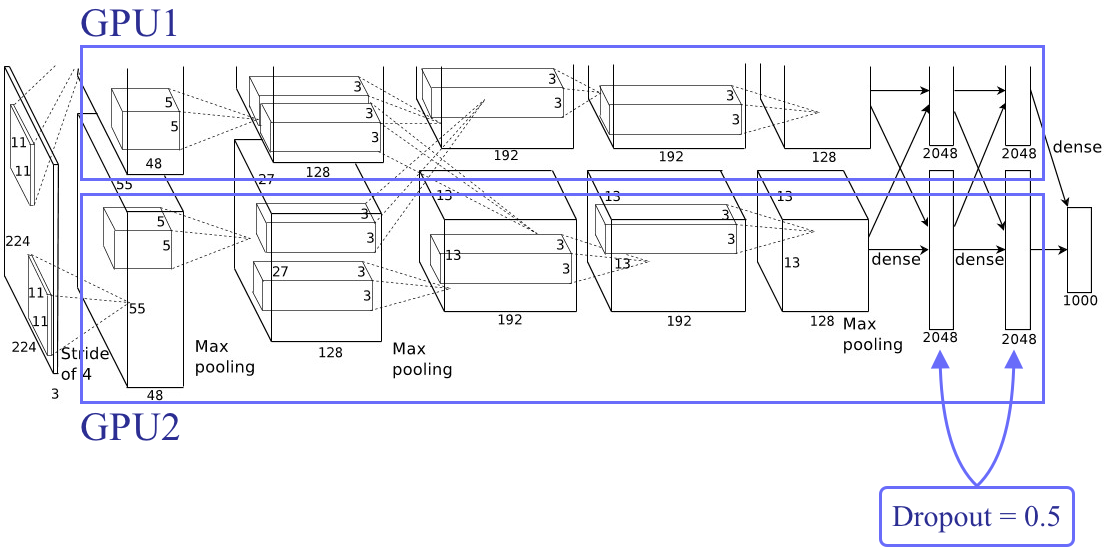
\includegraphics[keepaspectratio, scale=0.2]{pic/alexnet_annot}
		\end{center}
	\end{figure}
	\vspace{-0.2cm}
    \begin{itemize}
   		\setlength{\itemsep}{-1.6pt}
        \item Training: 6 days on 2 NVIDIA GTX 580 GPUs (3 GB RAM)
        \item 8 layers / 60 million parameters and 650,000 neurons
        \item 5 convolutional layers, some of which are followed by max-pooling layers
        \item 3 fully-connected layers
        \item Testing: Multi-crop
        \begin{itemize}
   	   		\setlength{\itemsep}{-1.6pt}
        	\item Classify different shifts of the image and vote over the lot!
        	\item Test-time data augmentation
        \end{itemize}
    \end{itemize}
\end{frame}

\begin{frame}{AlexNet Architecture}
	\textcolor[rgb]{0.998, 0.007, 0.003}{CONV1} \newline
	\textcolor[rgb]{0.001, 0.001, 0.998}{MAX POOL1} \newline
	\textcolor[rgb]{0.219, 0.463, 0.114}{NORM1} \newline 
	\textcolor[rgb]{0.998, 0.007, 0.003}{CONV2} \newline
	\textcolor[rgb]{0.001, 0.001, 0.998}{MAX POOL2} \newline
	\textcolor[rgb]{0.219, 0.463, 0.114}{NORM2} \newline 
	\textcolor[rgb]{0.998, 0.007, 0.003}{CONV3} \newline
	\textcolor[rgb]{0.998, 0.007, 0.003}{CONV4} \newline
	\textcolor[rgb]{0.998, 0.007, 0.003}{CONV5} \newline
	\textcolor[rgb]{0.001, 0.001, 0.998}{MAX POOL3} \newline
	\textcolor[rgb]{0.902, 0.570, 0.218}{FC6} \newline
	\textcolor[rgb]{0.902, 0.570, 0.218}{FC7} \newline
	\textcolor[rgb]{0.902, 0.570, 0.218}{FC8}
	
	\begin{textblock*}{5cm}(3.7cm,3cm) % {block width} (coords)
		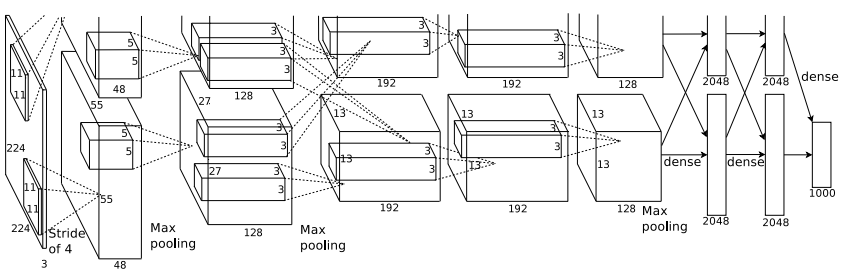
\includegraphics[keepaspectratio, scale=0.4]{pic/alexnet}
	\end{textblock*}
\end{frame}

\begin{frame}{AlexNet Architecture}
	\vspace{0.5cm}
	Input: $227 \times 227 \times 3$ images \vspace{0.3cm} \newline 
	\textbf{First layer} (CONV1): 96 $11 \times 11$ filters applied at stride 4 \hspace{2cm} $W^{\prime} = \frac{W - F + 2P}{S + 1}$ \newline
	$\Rightarrow$ \color{blue} Q: what is the output volume size? Hint: (227-11)/4+1 = 55
	
	\begin{textblock*}{5cm}(8.3cm,1.3cm) % {block width} (coords)
	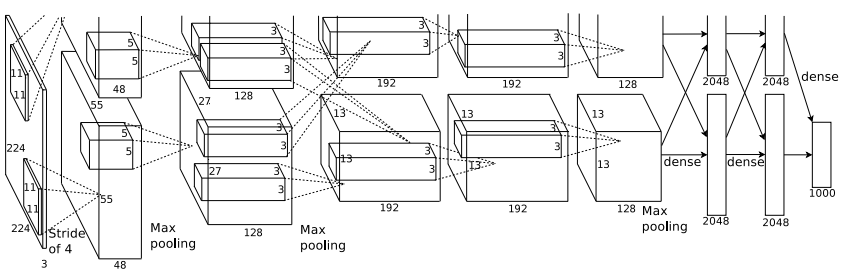
\includegraphics[keepaspectratio, scale=0.25]{pic/alexnet}
	\end{textblock*}
\end{frame}

\begin{frame}{AlexNet Architecture}
	\vspace{0.5cm}
	Input: $227 \times 227 \times 3$ images \vspace{0.3cm} \newline
	\textbf{First layer} (CONV1): 96 $11 \times 11$ filters applied at stride 4 \hspace{2cm} $W^{\prime} = \frac{W - F + 2P}{S + 1}$ \newline 
	$\Rightarrow$ Output volume [$55 \times 55 \times 96$]

	\begin{textblock*}{5cm}(8.3cm,1.3cm) % {block width} (coords)
		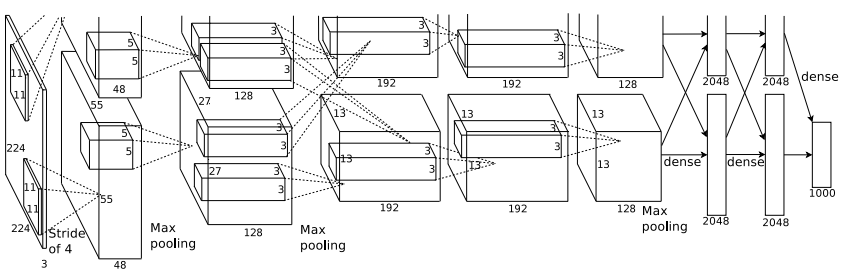
\includegraphics[keepaspectratio, scale=0.25]{pic/alexnet}
	\end{textblock*}
	\begin{textblock*}{6cm}(9cm,5cm) % {block width} (coords)
		\begin{figure}
			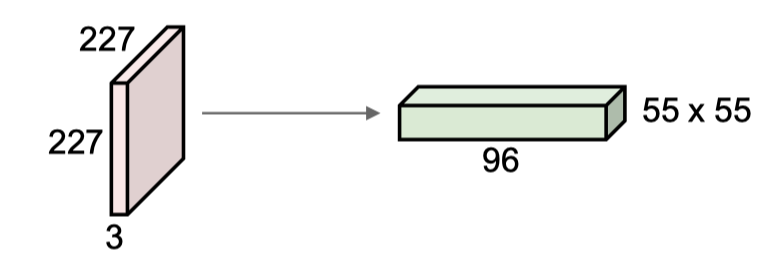
\includegraphics[keepaspectratio, scale=0.25]{pic/cnn_layer}
			\vspace{-2em}
			\caption*{\hspace{1cm} {\scriptsize Figure: Alex Krizhevsky, et al., 2012}}
		\end{figure}

	\end{textblock*}
\end{frame}

\begin{frame}{AlexNet Architecture}
	\vspace{1cm}
	Input: $227 \times 227 \times 3$ images \vspace{0.3cm} \newline 
	\textbf{First layer} (CONV1): 96 $11 \times11$ filters applied at stride 4 \newline 
	$\Rightarrow$ Output volume [$55 \times 55 \times 96$] \newline
	\color{blue} Q: What is the total number of parameters in this layer?
	
	\begin{textblock*}{5cm}(8.3cm,1.3cm) % {block width} (coords)
	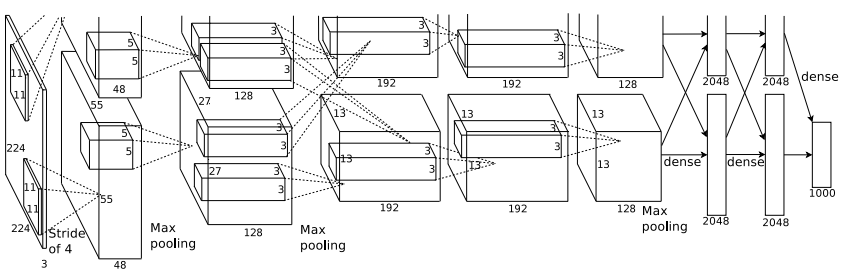
\includegraphics[keepaspectratio, scale=0.25]{pic/alexnet}
	\end{textblock*}
	
	\begin{textblock*}{6cm}(10cm,3.5cm) % {block width} (coords)
		\begin{figure}
			\centering
			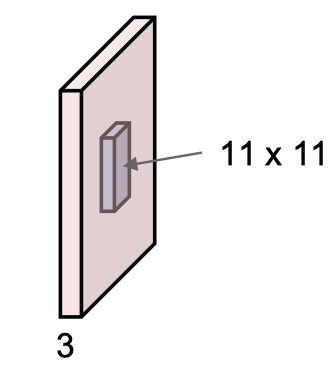
\includegraphics[keepaspectratio, scale=0.25]{pic/cnn_layer2}
			\caption*{\scriptsize{Figure: Alex Krizhevsky, et al., 2012}}
		\end{figure}
	\end{textblock*}
\end{frame}

\begin{frame}{AlexNet Architecture}
	\vspace{1cm}
	Input: $227 \times 227 \times 3$ images \vspace{0.3cm} \newline 
	\textbf{First layer} (CONV1): 96 $11 \times11$ filters applied at stride 4 \newline 
	$\Rightarrow$ Output volume [$55 \times 55 \times 96$] \newline
	Parameters: $(11 \times 11 \times 3 + 1) \times 96 = 35K$
	
	\begin{textblock*}{5cm}(8.3cm,1.3cm) % {block width} (coords)
		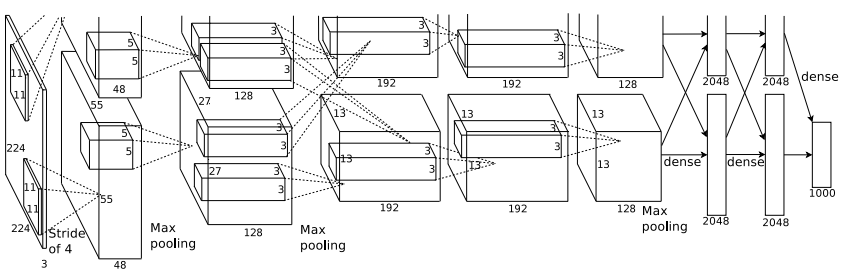
\includegraphics[keepaspectratio, scale=0.25]{pic/alexnet}
	\end{textblock*}
	
	\begin{textblock*}{6cm}(10cm,3.5cm) % {block width} (coords)
		\begin{figure}
			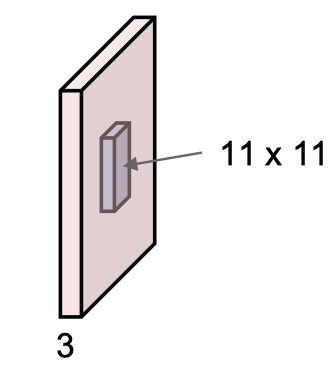
\includegraphics[keepaspectratio, scale=0.25]{pic/cnn_layer2}
			\caption*{\scriptsize{Figure: Alex Krizhevsky, et al., 2012}}
		\end{figure}
	\end{textblock*}
\end{frame}

\begin{frame}{AlexNet Architecture}
	\vspace{1cm}
	Input: $227 \times 227 \times 3$ images \newline 
	After CONV1: $55 \times 55 \times 96$ \vspace{0.3cm} \newline
	\textbf{Second layer} (POOL1): $3 \times 3$ filters applied at stride 2 \hspace{2cm} $W^{\prime} = \frac{W - F + 2P}{S + 1}$ \newline 
	\color{blue} Q: What is the output volume size? Hint: (55-3)/2+1 = 27
	
	\begin{textblock*}{5cm}(8.3cm,1.3cm) % {block width} (coords)
		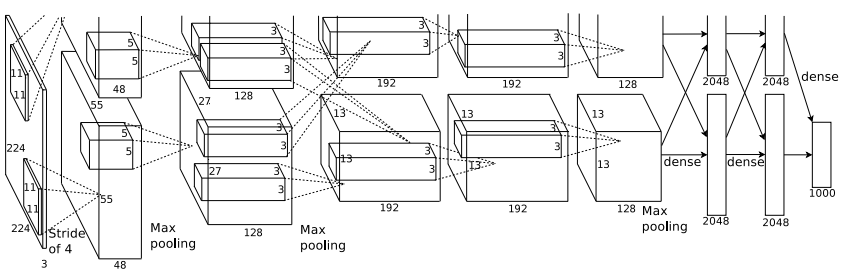
\includegraphics[keepaspectratio, scale=0.25]{pic/alexnet}
	\end{textblock*}
\end{frame}

\begin{frame}{AlexNet Architecture}
	\vspace{1cm}
	Input: $227 \times 227 \times 3$ images \newline 
	After CONV1: $55 \times 55 \times 96$ \vspace{0.3cm} \newline
	\textbf{Second layer} (POOL1): $3 \times 3$ filters applied at stride 2 
	\hspace{2cm} $W^{\prime} = \frac{W - F + 2P}{S + 1}$ \newline 
	Output volume: $27 \times 27 \times 96$ \vspace{0.3cm} \newline
	\color{blue} Q: What is the number of parameters in this layer?
	
	\begin{textblock*}{5cm}(8.3cm,1.3cm) % {block width} (coords)
		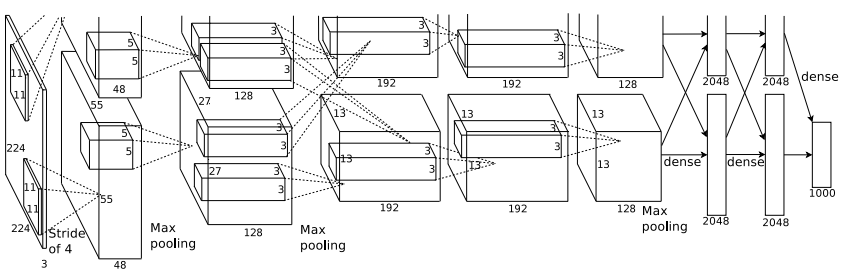
\includegraphics[keepaspectratio, scale=0.25]{pic/alexnet}
	\end{textblock*}
\end{frame}

\begin{frame}{AlexNet Architecture}
	\vspace{1cm}
	Input: $227 \times 227 \times 3$ images \newline 
	After CONV1: $55 \times 55 \times 96$ \vspace{0.3cm} \newline
	\textbf{Second layer} (POOL1): $3 \times 3$ filters applied at stride 2 \newline 
	Output volume: $27 \times 27 \times 96$ \newline
	Parameters: 0!
	
	\begin{textblock*}{5cm}(8.3cm,1.3cm) % {block width} (coords)
		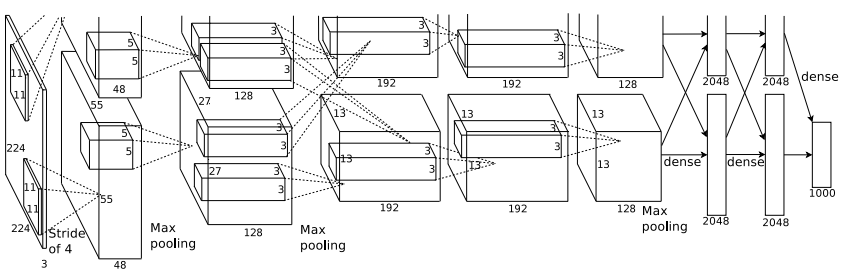
\includegraphics[keepaspectratio, scale=0.25]{pic/alexnet}
	\end{textblock*}
\end{frame}

\begin{frame}{AlexNet Full Architecture}
	[$227 \times 227 \times 3$] INPUT \newline
	[$55 \times 55 \times 96$] \textcolor[rgb]{0.998, 0.007, 0.003}{CONV1}: 96 $11 \times 11$ filters at stride 4, pad 0 \newline
	[$27 \times 27 \times 96$] \textcolor[rgb]{0.001, 0.001, 0.998}{MAX POOL1}: MAX POOL1: $3 \times 3$ filters at stride 2 \newline
	[$27 \times 27 \times 96$] \textcolor[rgb]{0.219, 0.463, 0.114}{NORM1}: Normalization layer \newline
	[$27 \times 27 \times 256$] \textcolor[rgb]{0.998, 0.007, 0.003}{CONV2}: 256 $5 \times 5$ filters at stride 1, pad 2 \newline
	[$13 \times 13 \times 256$] \textcolor[rgb]{0.001, 0.001, 0.998}{MAX POOL2}: $3 \times 3$ filters at stride 2 \newline
	[$13 \times 13 \times 256$] \textcolor[rgb]{0.219, 0.463, 0.114}{NORM2}: Normalization layer \newline 
	[$13 \times 13 \times 384$] \textcolor[rgb]{0.998, 0.007, 0.003}{CONV3}: 384 $3 \times 3$ filters at stride 1, pad 1 \newline
	[$13 \times 13 \times 384$] \textcolor[rgb]{0.998, 0.007, 0.003}{CONV4}: 384 $3 \times 3$ filters at stride 1, pad 1 \newline
	[$13 \times 13 \times 256$] \textcolor[rgb]{0.998, 0.007, 0.003}{CONV5}: 256 $3 \times 3$ filters at stride 1, pad 1 \newline
	[$6 \times 6 \times 256]$ \textcolor[rgb]{0.001, 0.001, 0.998}{MAX POOL3}: $3 \times 3$ filters at stride 2 \newline
	[$4096$] \textcolor[rgb]{0.902, 0.570, 0.218}{FC6} 4096 neurons \newline
	[$4096$] \textcolor[rgb]{0.902, 0.570, 0.218}{FC7} 4096 neurons \newline
	[$1000$] \textcolor[rgb]{0.902, 0.570, 0.218}{FC8} 1000 neurons (class scores) 

	\begin{textblock*}{5cm}(8.7cm, 6.4cm) % {block width} (coords)
		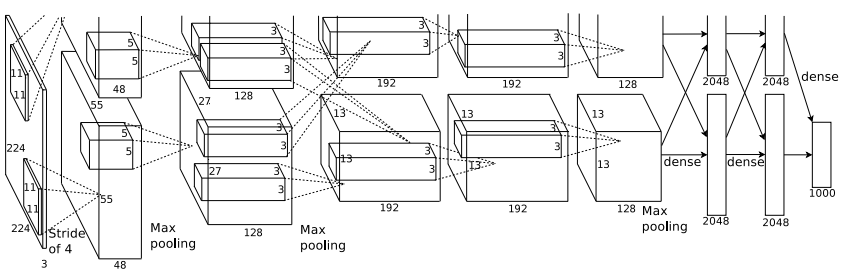
\includegraphics[keepaspectratio, width=7cm]{pic/alexnet}
	\end{textblock*}
\end{frame}


\begin{frame}{Dropout}
	\begin{itemize}
		\item In each forward pass, randomly set some neurons to zero
		\setbeamertemplate{itemize subitem}{$\rightarrow$}
		\begin{itemize}
			\item Probability of dropping is a hyperparameter; 0.5 is common
		\end{itemize}
		\begin{figure}[htpb]
			\begin{center}
				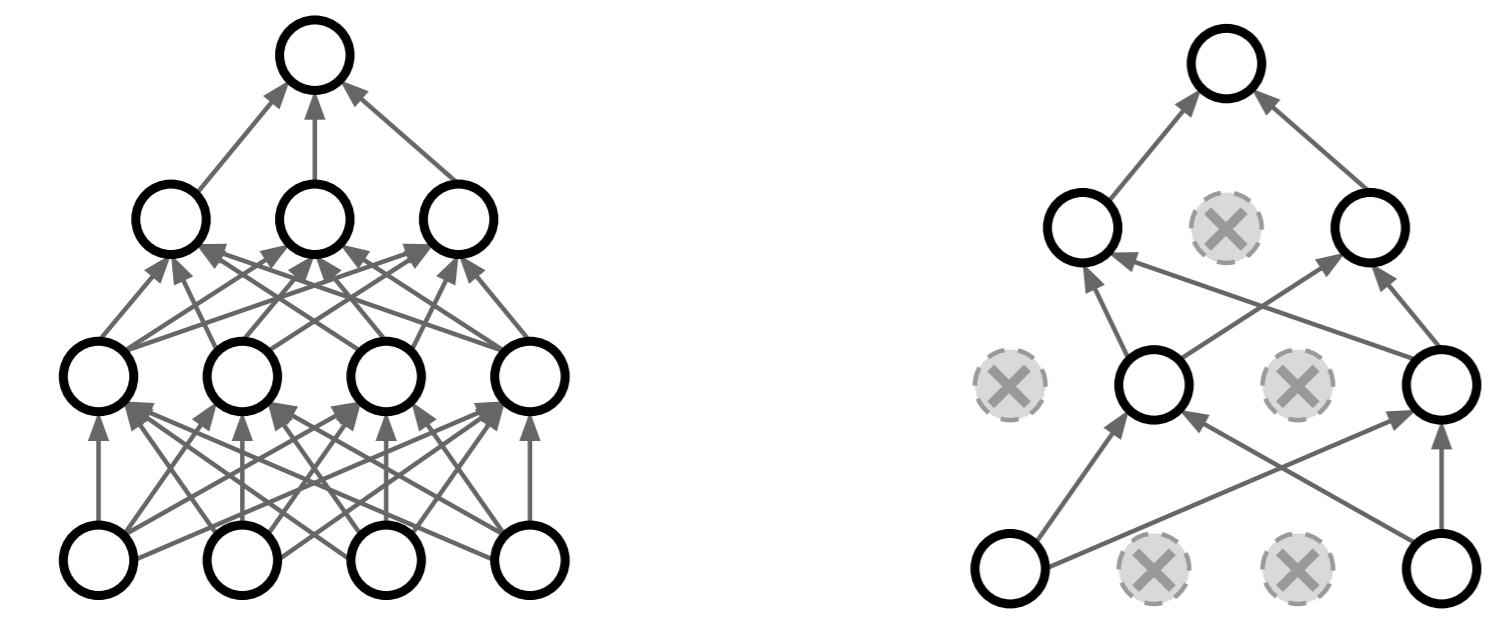
\includegraphics[keepaspectratio, scale=0.15]{pic/dropout}
				\caption*{\scriptsize Srivastava et al., JMLR 2014}
			\end{center}
		\end{figure}
		\vspace{-1em}
		\item Thus, a smaller network is trained for each sample
		\setbeamertemplate{itemize subitem}{$\rightarrow$}
		\begin{itemize}
			\item Smaller network provides a regularization effect
		\end{itemize}
	\end{itemize}
\end{frame}

\begin{frame}{Dropout}
	\begin{itemize}
		\item How can dropout be a good idea?
	\end{itemize}
	\begin{figure}[htpb]
		\begin{center}
			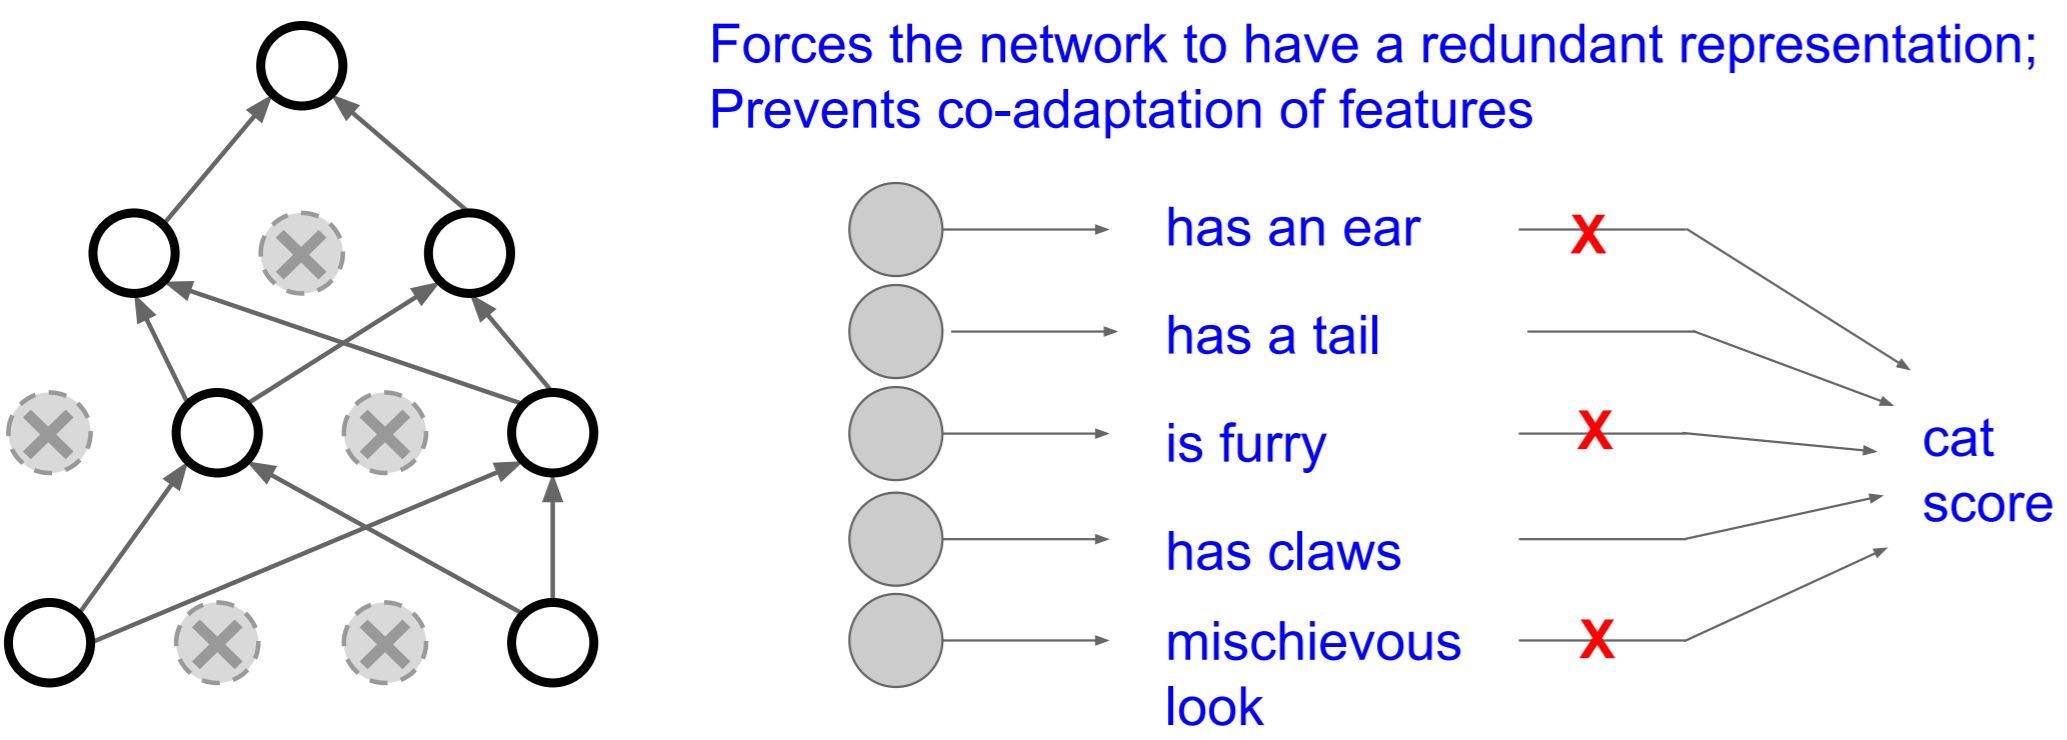
\includegraphics[keepaspectratio, scale=0.15]{pic/dropout2}
			\caption*{\scriptsize Hinton et al., 2012}
		\end{center}
	\end{figure}
\end{frame}

\begin{frame}{Dropout}
	\begin{itemize}
		\item During training: Backpropagation is effectively performed only over the remaining network
		\setbeamertemplate{itemize subitem}{$\rightarrow$}
		\begin{itemize}
			\item The effective network is different for different inputs
			\item Gradients are obtained only for the weights and biases from “On” nodes to “On” nodes
			\item For the remaining, the gradient is just 0
		\end{itemize}
	\end{itemize}
	
	\begin{figure}[htpb]
		\begin{center}
			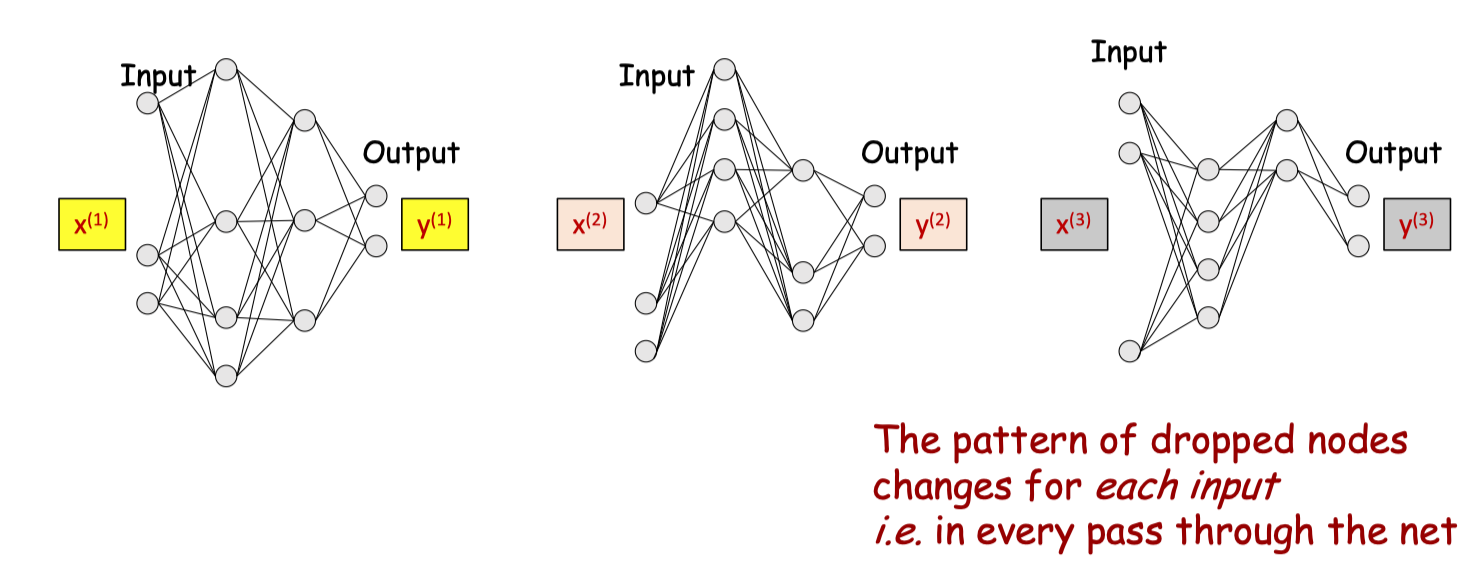
\includegraphics[keepaspectratio, scale=0.23]{pic/dropout3}
		\end{center}
	\end{figure}
\end{frame}

\begin{frame}{Dropout}
	\begin{itemize}
		\item Test error for different architectures on MNIST with and without dropout
		\setbeamertemplate{itemize subitem}{$\rightarrow$}
		\begin{itemize}
			\item 2-4 hidden layers with 1024-2048 units
		\end{itemize}
	\end{itemize}
	\begin{figure}[htpb]
		\begin{center}
			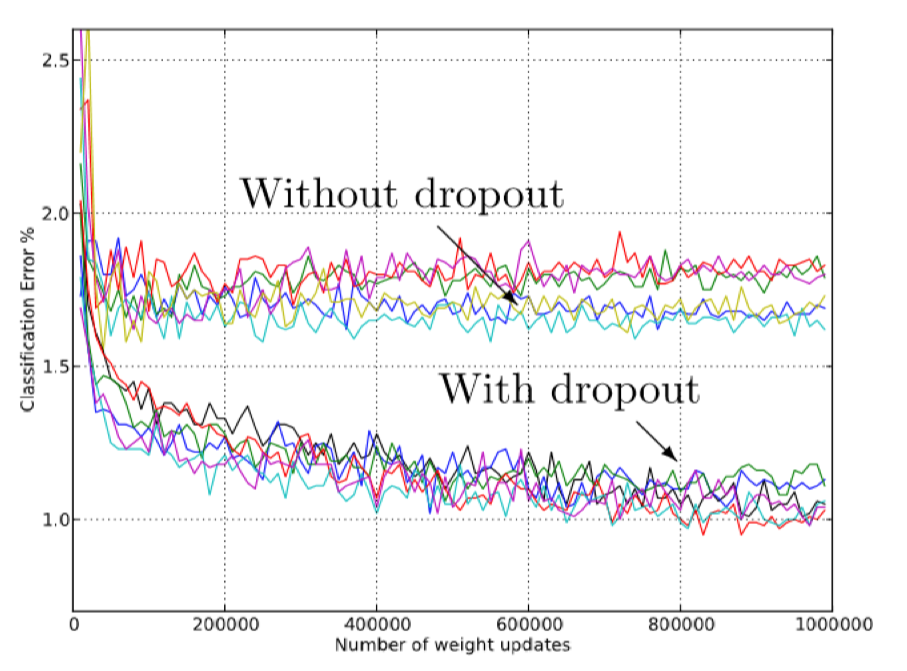
\includegraphics[keepaspectratio, scale=0.22]{pic/dropout4}
			\caption*{\scriptsize Srivastava et al., 2013}
		\end{center}
	\end{figure}
\end{frame}

\begin{frame}{Flashback To Activation Functions}
%	\setbeamercolor{item}{fg=blue}      
	\setbeamercolor{itemize subitem}{fg=red}
	
	\textbf{Sigmoid:} 
	\begin{itemize}
		\item $\sigma(x) = \frac{1}{1+e^{-x}}$
		\item Squashes numbers to range [0,1]
		\item Historically popular since they have nice interpretation \newline as a saturating “firing rate” of a neuron
		\item[\textcolor{red}{$\bullet$}] \color{red} \textbf{Problems:}
		\setbeamertemplate{itemize subitem}{$\rightarrow$}
		\begin{itemize}
			\item \color{red} Saturated neurons “kill” the gradients
			\item \color{red} Sigmoid outputs are not zero-centered
		\end{itemize}
	\end{itemize}
	\textbf{Tanh:}
	\begin{itemize}
		\item $tanh(x) = \frac{1-e^{-2x}}{1+e^{2x}} = 1 - 2\sigma(2x)$
		\item Squashes numbers to range [-1,1]
		\item Zero centered (nice)
		\item[\textcolor{red}{$\bullet$}] \color{red} Still kills gradients when saturated
	\end{itemize}
	\begin{textblock*}{5cm}(11cm,1.6cm) % {block width} (coords)
	\begin{figure}[htbp]
		\begin{center}
			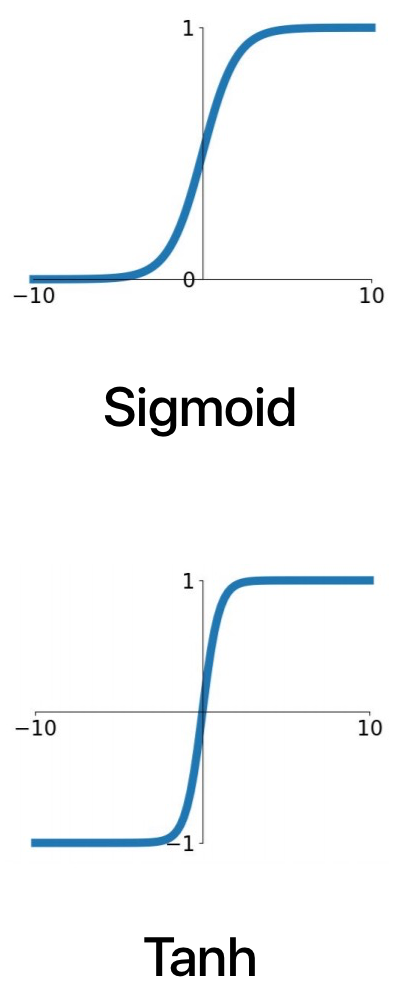
\includegraphics[keepaspectratio, scale=0.18]{pic/sigmoid_tanh}
		\end{center}
	\end{figure}
	\end{textblock*}
	
\end{frame}

\begin{frame}{ReLU}
	\setbeamercolor{itemize subitem}{fg=red}
	\setbeamercolor{itemize subsubitem}{fg=red}
	\textbf{ReLU}
	\begin{itemize}
		\item Does not saturate (in +region)
		\item Very computationally efficient
		\item Converges much faster than sigmoid/tanh \newline in practice (e.g. 6x)
		\item Actually more biologically plausible than sigmoid
		\item[\textcolor{red}{$\bullet$}] \color{red} \textbf{Problems:}
		\setbeamertemplate{itemize subitem}{$\rightarrow$}
		\begin{itemize}
			\item \color{red} Not zero-centered output
			\item \color{red} An annoyance:
			\setbeamertemplate{itemize subsubitem}{$\star$}
			\begin{itemize}
				\item \color{red} hint: what is the gradient when x < 0?
			\end{itemize}
		\end{itemize}
	\end{itemize}
	\begin{textblock*}{5cm}(11cm,2.5cm) % {block width} (coords)
		\begin{figure}[htbp]
			\begin{center}
				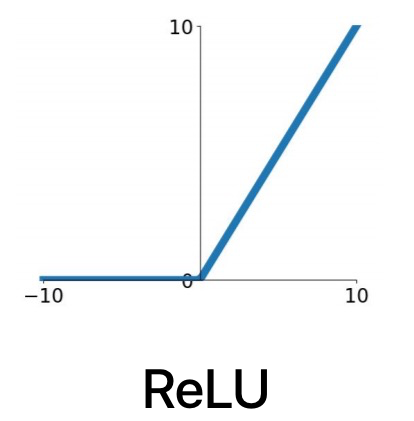
\includegraphics[keepaspectratio, scale=0.3]{pic/ReLU}
			\end{center}
		\end{figure}
	\end{textblock*}
\end{frame}

\begin{frame}{ReLU}
	\begin{itemize}
		\item ReLu trains faster than tanh
	\end{itemize}
	\begin{figure}[htbp]
		\begin{center}
			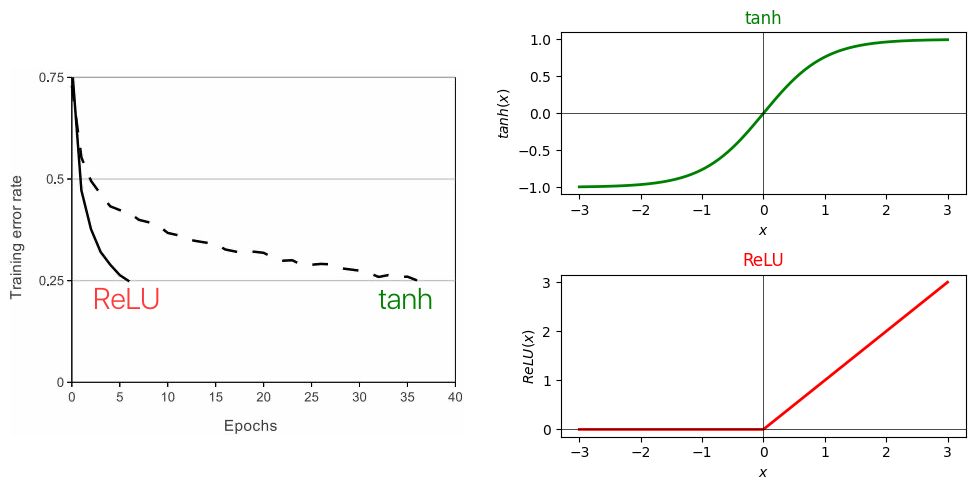
\includegraphics[keepaspectratio, scale=0.3]{pic/relu_faster}
			\caption*{\scriptsize Krizhevsky, et al., 2012}
		\end{center}
	\end{figure}
\end{frame}

\begin{frame}{ReLU Initialization}
	\begin{itemize}
		\item people like to initialize ReLU neurons with slightly positive biases (e.g. 0.01)
		\item It can be due initialization or high learning rate
	\end{itemize}
	\begin{figure}[htpb]
		\begin{center}
			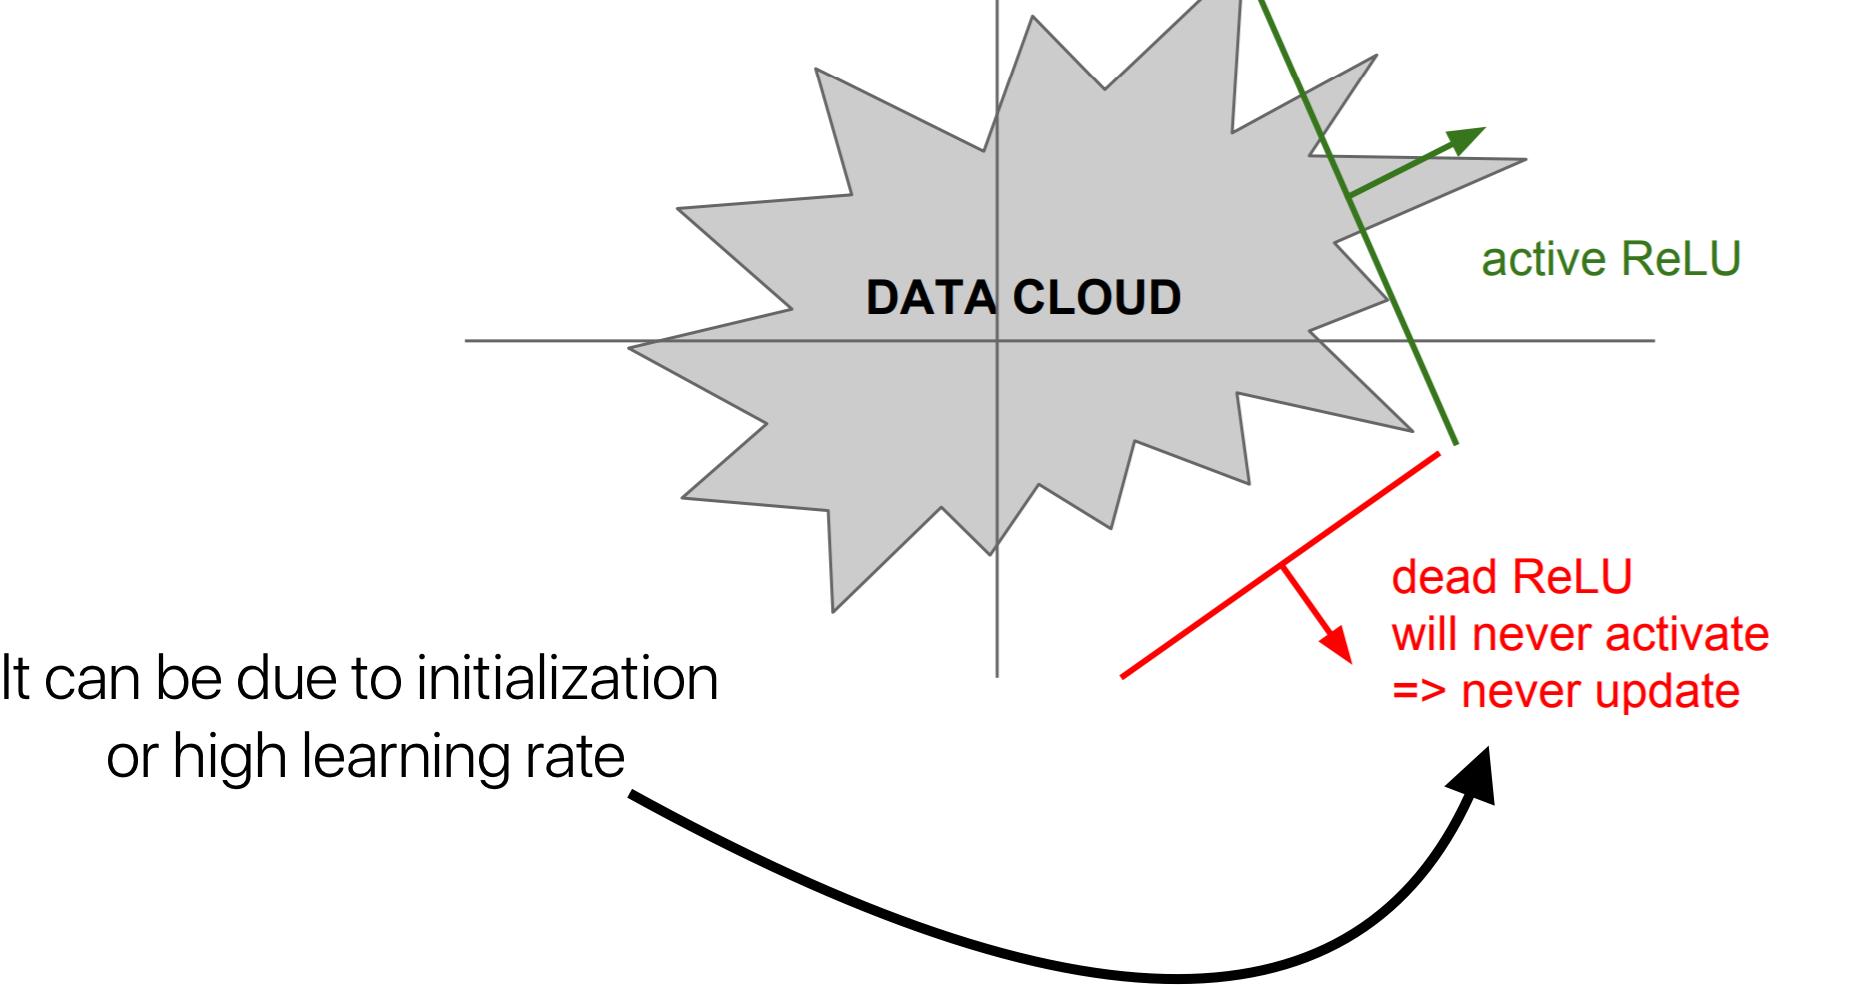
\includegraphics[keepaspectratio, scale=0.15]{pic/dead_relu}
		\end{center}
	\end{figure}
\end{frame}

\begin{frame}{Learning magic in Alexnet}
	\begin{itemize}
		\item First use of ReLU
		\setbeamertemplate{itemize subitem}{$\rightarrow$}
		\begin{itemize}
			\item Made a large difference in convergence
		\end{itemize}
		\item "Dropout" – 0.5 (in FC layers only)
		\item Heavy data augmentation
		\item SGD Momentum 0.9 with mini batch size 128
		\item L2 weight decay 5e-4
		\item Learning rate: 0.01, decreased by 10 every time validation accuracy plateaus
		\item Evaluated using: Validation accuracy
		\item \textbf{Final top-5 error: 18.2\% with a single net, 15.4\% using an ensemble of 7 networks}
		\setbeamertemplate{itemize subitem}{$\rightarrow$}
		\begin{itemize}
			\item \textbf{Lowest prior error using conventional classifiers: > 25 \%}
		\end{itemize}
	\end{itemize}
\end{frame}

\section{ResNet}

\begin{frame}
	\begin{figure}[htpb]
		\begin{center}
			
\includegraphics[keepaspectratio, scale=0.5]{pic/deeper}
		\end{center}
	\end{figure}
\end{frame}

\begin{frame}{Revolution of Depth}
	\begin{figure}[htpb]
		\begin{center}
			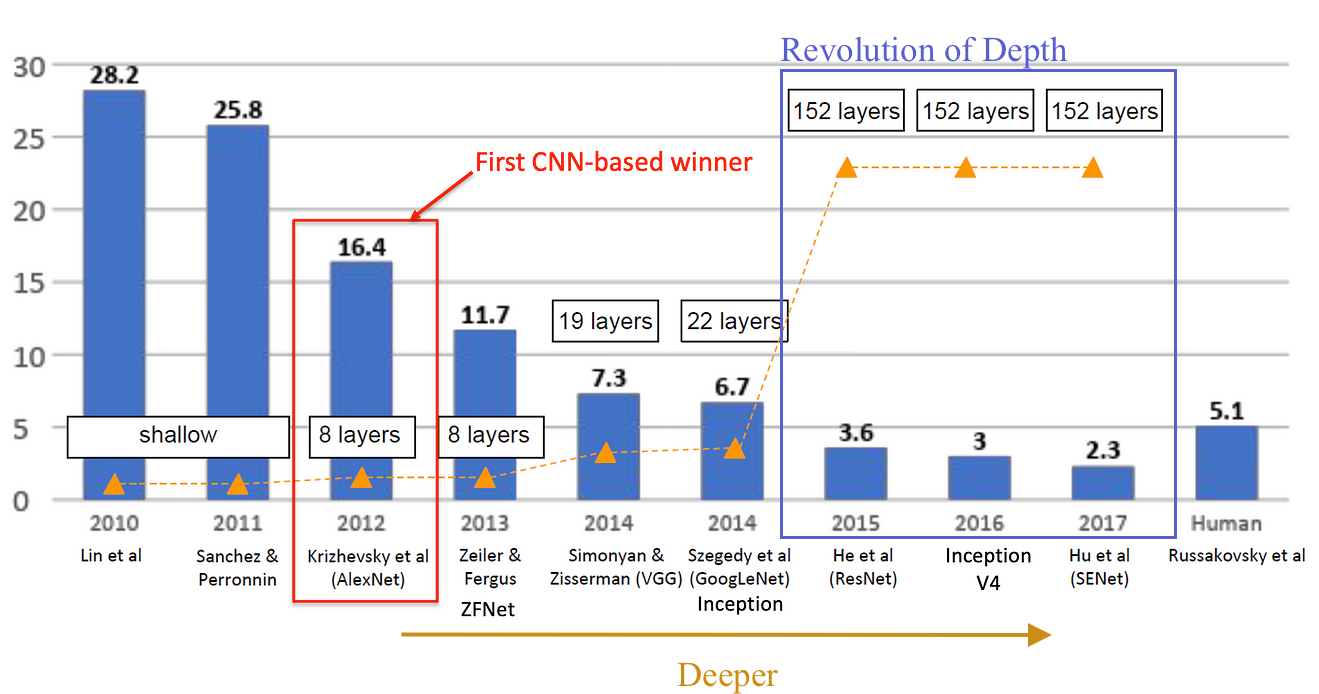
\includegraphics[keepaspectratio, scale=0.25]{pic/resnet-chart}
		\end{center}
	\end{figure}
\end{frame}

\begin{frame}{ResNet [He, et al., (2015)]}
	
	\begin{textblock*}{5cm}(10.5cm,1.3cm) % {block width} (coords)
		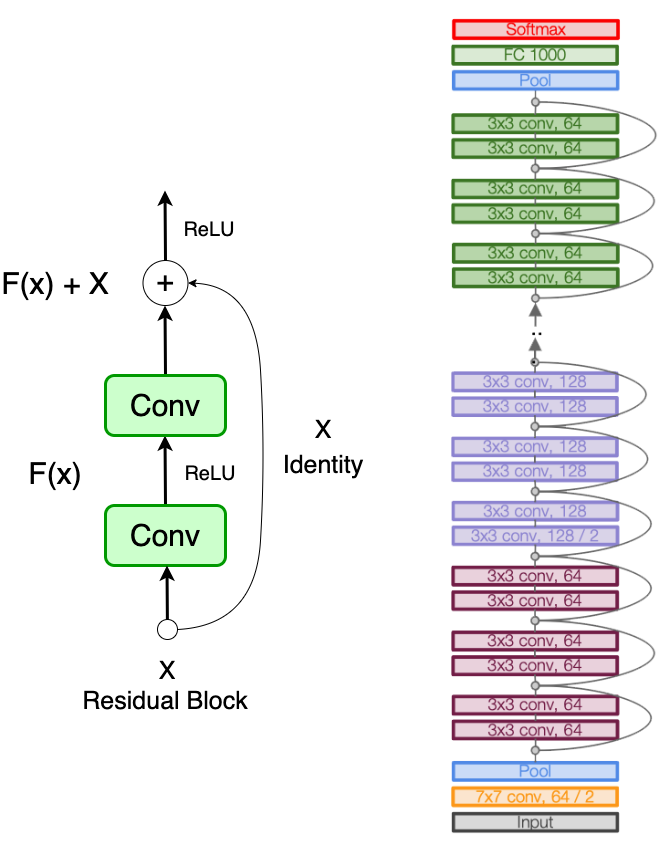
\includegraphics[keepaspectratio, scale=0.23]{pic/resBlock}
	\end{textblock*}
	
	\begin{itemize}
		\item \color{red} Very deep networks using residual connections
		\item \color{blue} ResNet introduces the concept of \color{red}{skip connections \newline (or residual connections)} \color{blue} that allow the gradient to \newline be directly backpropagated to earlier layers
		\item \color{blue} Skip connections help in overcoming the degradation \newline problem, where the accuracy saturates and then \newline degrades rapidly as the network depth increases.
		\item \color{blue} 152-layer model for ImageNet
		\item \color{blue} ILSVRC’15 classification winner (3.57 \% top 5 error)
		\item \color{blue} Swept all classification and detection competitions \newline in ILSVRC’15 and COCO’15!
	\end{itemize}
\end{frame}

\begin{frame}{ResNet [He, et al., (2015)]}
	\begin{itemize}
		\item What happens when we continue stacking deeper layers on a ``plain'' convolutional neural network?
		\item \textbf{Question}: What’s strange about these training and test curves?
	\end{itemize}
	\begin{figure}[htpb]
		\begin{center}
			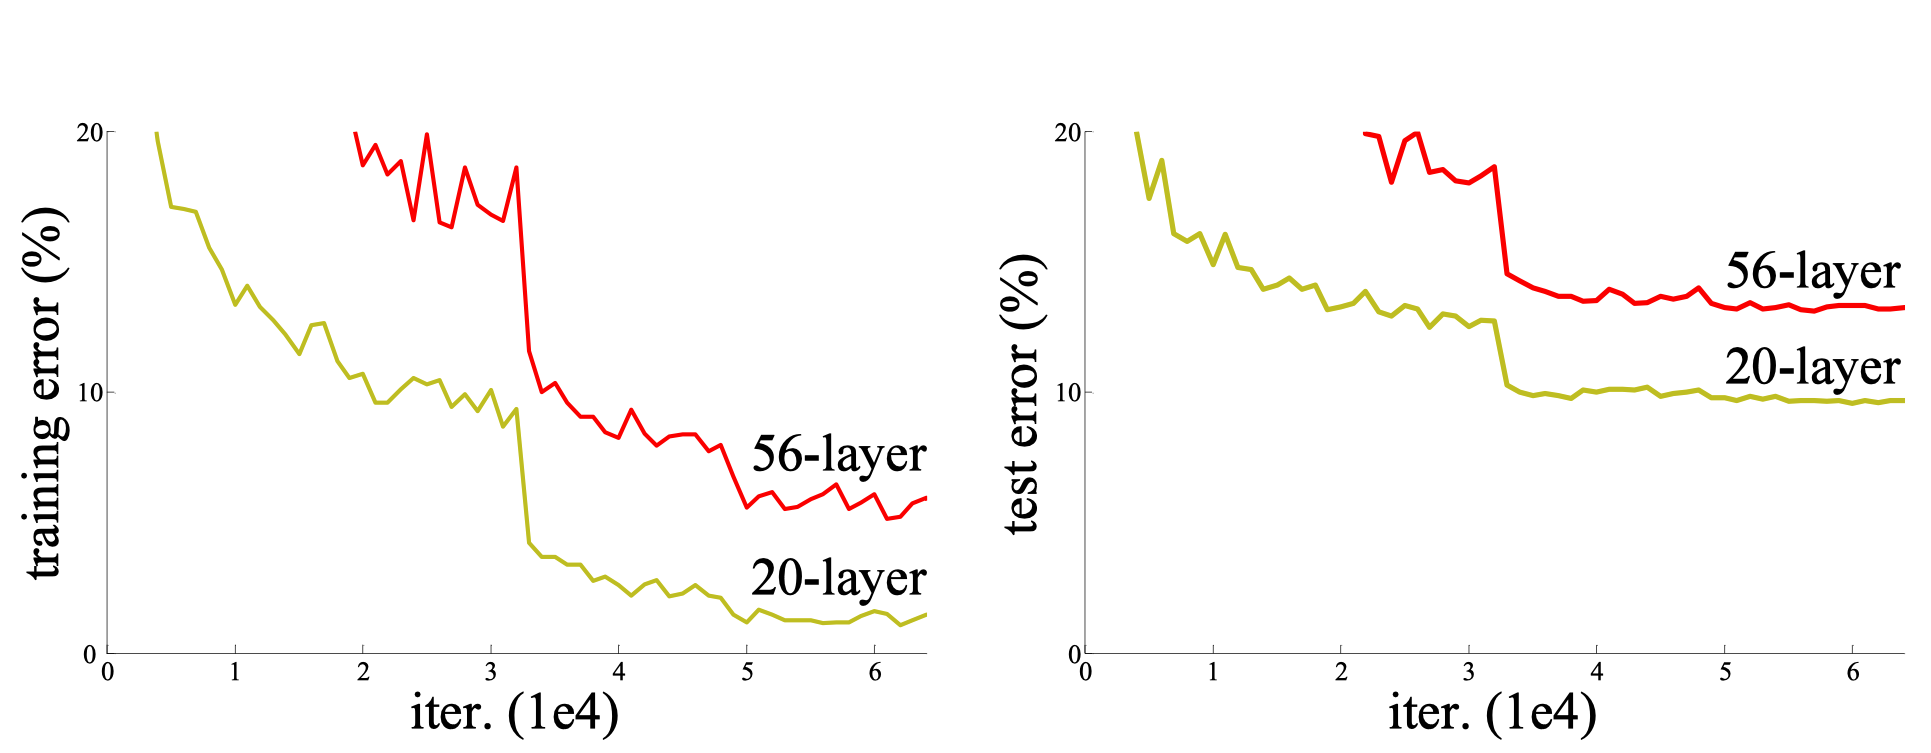
\includegraphics[keepaspectratio, scale=0.17]{pic/plain}
			\captionsetup{justification=centering}
			\caption*{\scriptsize{Training error (left) and test error (right) on CIFAR-10 with 20-layer and 56-layer “plain” networks}}
		\end{center}
	\end{figure}
\end{frame}

\begin{frame}{ResNet [He, et al., (2015)]}
	
	\begin{textblock*}{5cm}(11cm,2cm) % {block width} (coords)
		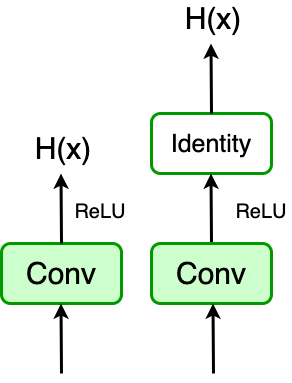
\includegraphics[keepaspectratio, scale=0.4]{pic/Identity}
	\end{textblock*}
	
	\begin{itemize}
		\item \textbf{\underline{Fact}:} Deeper models have more representation \newline power (more parameters) than shallower models.
		\item But \textbf{56-layer model performs worse} on both training \newline and test error and it’s not caused by overfitting!
		\item \textbf{Hypothesis:} the problem is an optimization problem, \newline deeper models are harder to optimize
		\item \color{red} What should the deeper model learn to be at least \newline as good as the shallower model?
		\item \color{red} A solution by construction is copying the learned \newline layers from the shallower model and setting additional \newline layers to identity mapping.
	\end{itemize}
\end{frame}

\begin{frame}{ResNet [He, et al., (2015)]}
	
	\begin{itemize}
		\item Solution: Use network layers to fit a residual mapping instead of directly trying to fit a desired underlying mapping
		\item Identity mapping: $H(x) = x \  \text{if} \ F(x) = 0$
%		\item Use layers to fit residual $F(x) = H(x) - x$ instead of H(x) directly
	\end{itemize}
	
	\begin{figure}[htpb]
		\begin{center}
			\hspace{2cm} 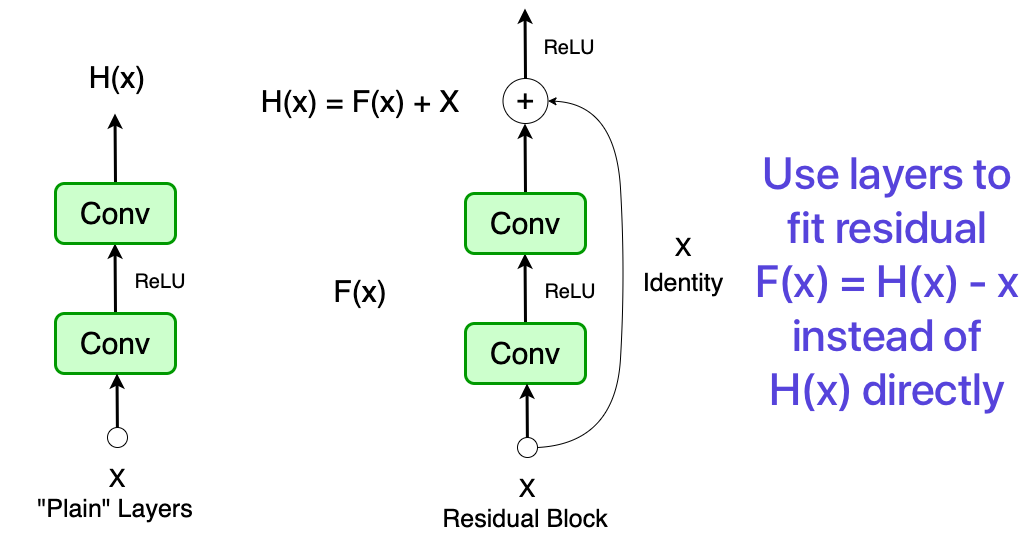
\includegraphics[keepaspectratio, scale=0.24]{pic/resBlock2}
		\end{center}
	\end{figure}

\end{frame}

\begin{frame}{Full ResNet architecture}
	\begin{textblock*}{5cm}(8.1cm,1.5cm) % {block width} (coords)
		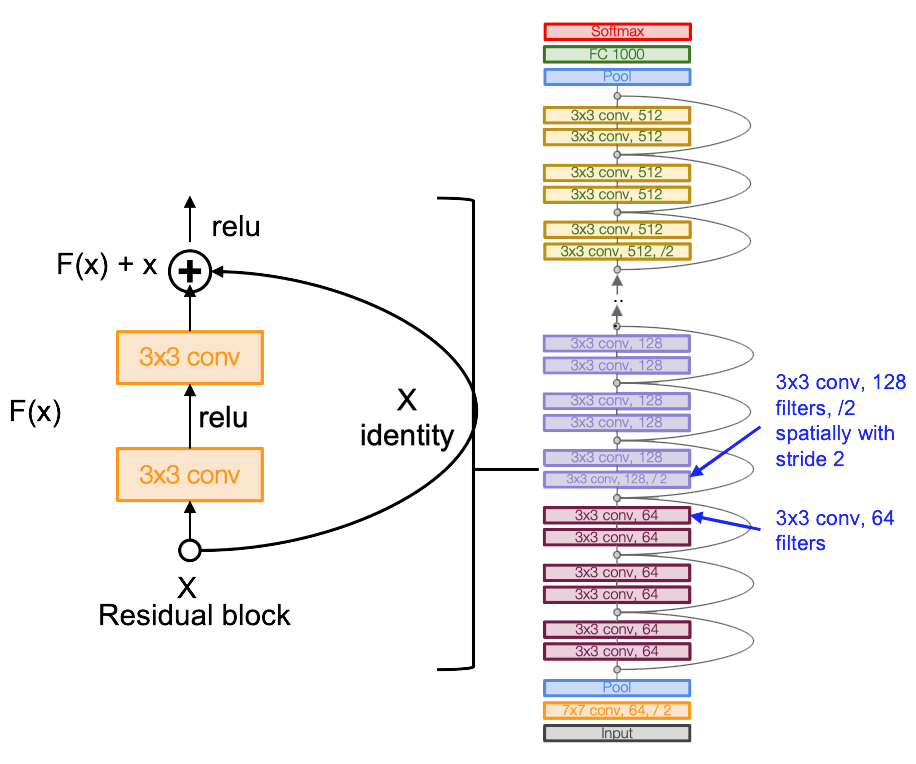
\includegraphics[keepaspectratio, scale=0.24]{pic/res_arch}
	\end{textblock*}
	
	\begin{itemize}
		\item Stack residual blocks
		\item Every residual block has two 3x3 conv layers
		\item Periodically, double number of filters \newline and downsample spatially using \newline stride 2 (/2 in each dimension) Reduce \newline the activation volume by half
		\item Additional conv layer at the beginning
		\item No FC layers at the end (only FC 1000 \newline to output classes)
		\item (In theory, you can train a ResNet with \newline input image of variable sizes)
	\end{itemize}
\end{frame}

\begin{frame}{Full ResNet architecture}
	\begin{textblock*}{5cm}(11cm,1.9cm) % {block width} (coords)
		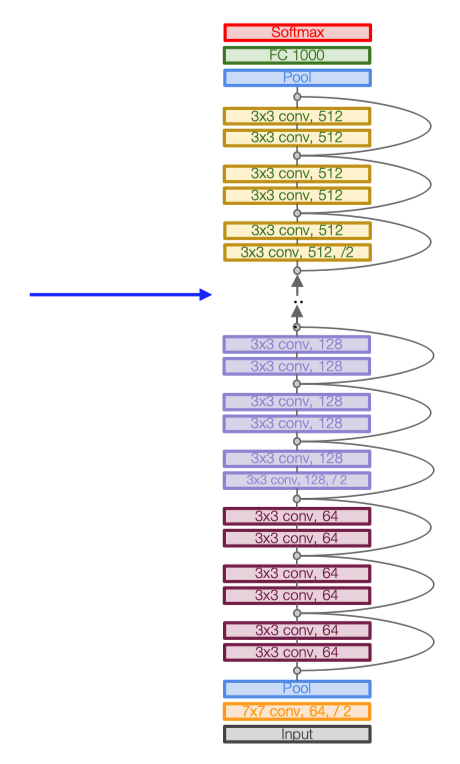
\includegraphics[keepaspectratio, scale=0.23]{pic/res_arch2}
	\end{textblock*}
	
	\begin{itemize}
		\item Total depths of 18, 34, 50, 101, or 152 layers for ImageNet
	\end{itemize}
\end{frame}

\begin{frame}{Full ResNet architecture}
	\begin{itemize}
		\item For deeper networks (ResNet- 50+), use “bottleneck” layer to improve efficiency (similar to GoogLeNet)
	\end{itemize}
	
	\begin{figure}[htpb]
		\begin{center}
			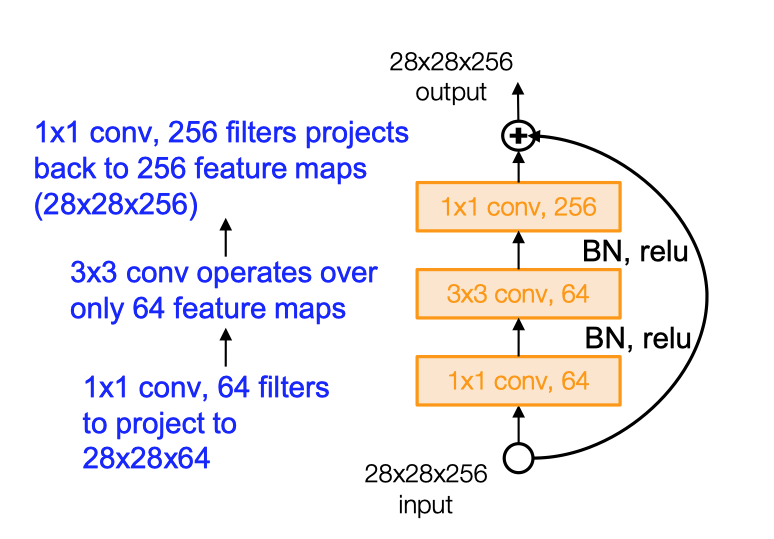
\includegraphics[keepaspectratio, scale=0.3]{pic/res_arch3}
		\end{center}
	\end{figure}
\end{frame}

\begin{frame}{Experimental Results}
	\begin{itemize}
		\item Able to train very deep networks without degrading (152 layers on ImageNet, 1202 on Cifar)
		\item Deeper networks now achieve lower training error as expected
		\item Swept 1st place in all ILSVRC and COCO 2015 competitions
	\end{itemize}
	
	\begin{figure}[htpb]
		\begin{center}
			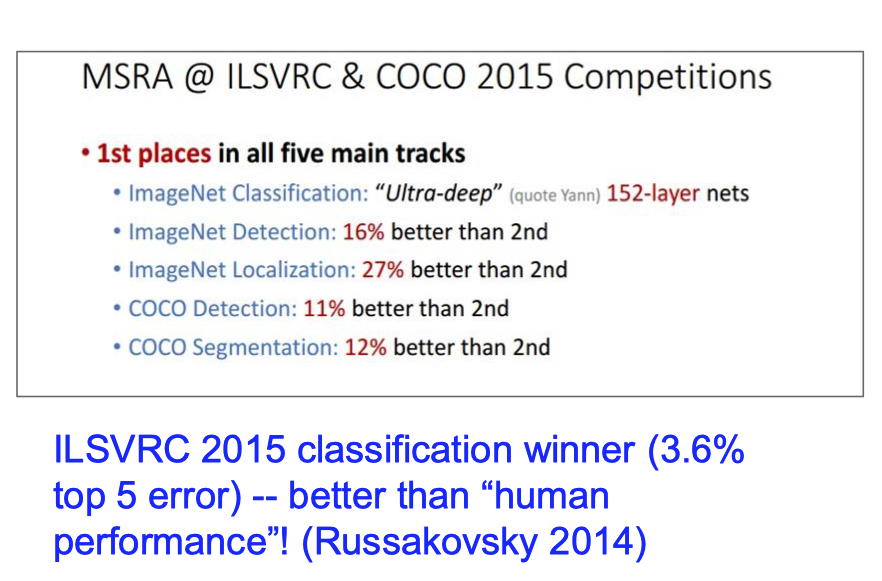
\includegraphics[keepaspectratio, scale=0.23]{pic/resnet_result}
		\end{center}
	\end{figure}
\end{frame}

\begin{frame}{ResNet Experiments}
	\begin{figure}[htpb]
		\begin{center}
			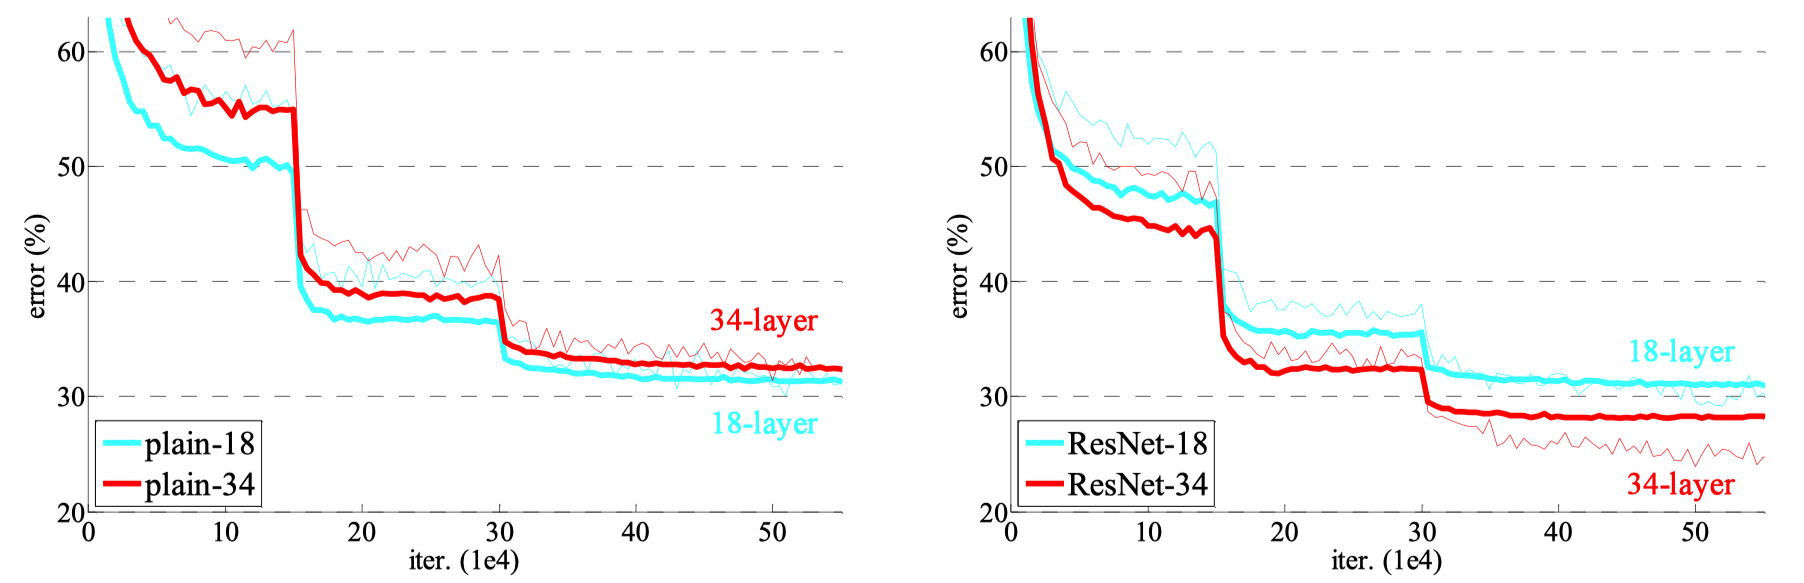
\includegraphics[keepaspectratio, scale=0.22]{pic/ResNetExp}
			\caption*{\scriptsize Thin curves denote training error, and bold curves denote validation error [He, et al. 2015]}
		\end{center}
	\end{figure}
\end{frame}

\begin{frame}{Training ResNet in practice:}
	\begin{itemize}
		\item Batch Normalization after every CONV layer
		\item Xavier initialization from He, et al.
		\item SGD + Momentum (0.9)
		\item Learning rate: 0.1, divided by 10 when validation error plateaus
		\item Mini-batch size 256
		\item Weight decay of 1e-5
		\item No dropout used
	\end{itemize}
\end{frame}

\begin{frame}{Key Points}
	\begin{itemize}
		\item \textbf{AlexNet} showed that you can use CNNs to train Computer Vision models. 
		\item \textbf{ResNet} showed us how to train extremely deep networks
		\setbeamertemplate{itemize subitem}{$\rightarrow$}
		\begin{itemize}
			\item Limited only by GPU \& memory!
			\item Showed diminishing returns as networks got bigger
		\end{itemize}
		\item After ResNet: CNNs were better than the human metric and focus shifted to other topics:
		\setbeamertemplate{itemize subitem}{$\star$}
		\begin{itemize}
			\item Efficient Networks: \textbf{MobileNet, ShuffleNet}
			\item \textbf{Neural Architecture Search} can now automate architecture design
		\end{itemize}
	\end{itemize}
\end{frame}

\begin{frame}{Model Comparison}
	\begin{figure}[htpb]
		\begin{center}
			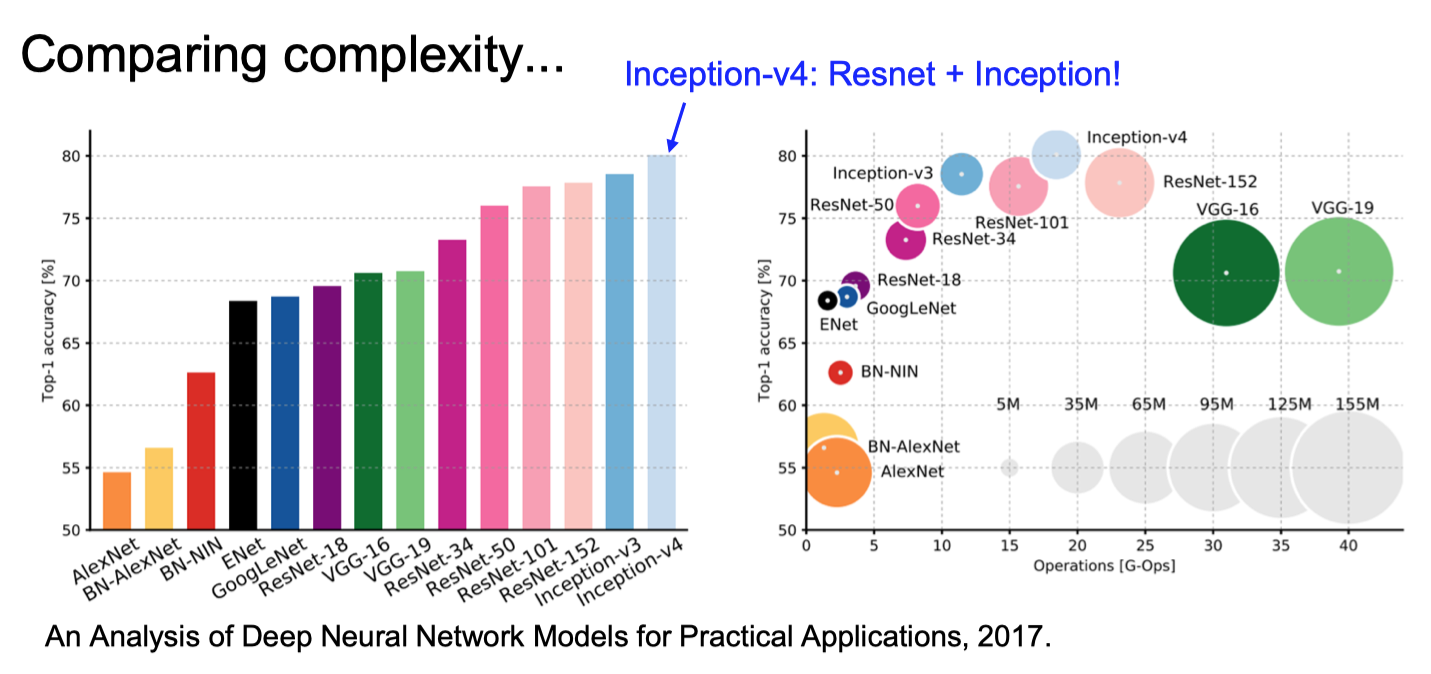
\includegraphics[keepaspectratio, scale=0.25]{pic/model_comp2}
			\caption*{}
		\end{center}
	\end{figure}
\end{frame}


\section{Data Preprocessing}

\begin{frame}{Normalizing the data}
	\begin{itemize}
		\item Assume $X_{n \times d}$ is data matrix, each sample in a row
		\item $i$ is the index of dimension (\ $i = 1, \dots d$\ )
	\end{itemize}
	\begin{figure}[htpb]
		\begin{center}
			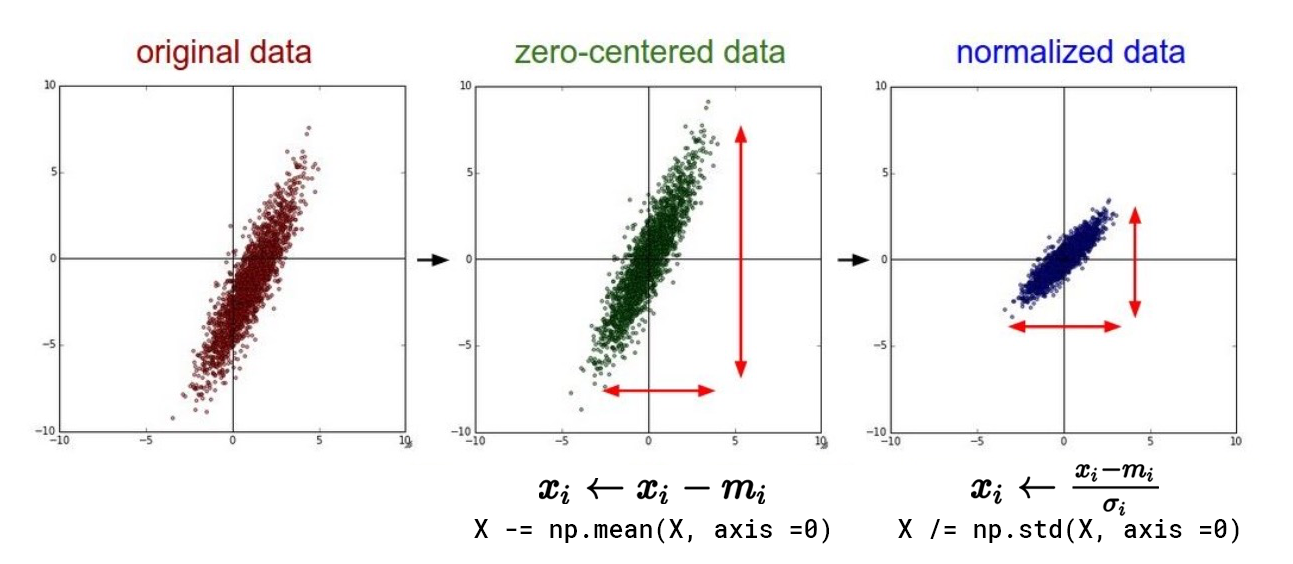
\includegraphics[keepaspectratio, scale=0.3]{pic/normaliz}
		\end{center}
	\end{figure}
\end{frame}

\begin{frame}{TLDR: In practice for Images: center only}
	\begin{itemize}
		\item Example: consider CIFAR-10 example with $[32,32,3]$ images
		\item 3 different approaches:
		\begin{enumerate}
		\item Subtract the mean image (e.g. AlexNet)
			\begin{itemize}
				\item mean image = $[32,32,3]$ array
			\end{itemize}
		\item Subtract per-channel mean (e.g. VGGNet)
			\begin{itemize}
				\item mean along each channel = 3 numbers
			\end{itemize}		
		\item Subtract per-channel mean and divide by per-channel std (e.g. ResNet)
		\end{enumerate}
	\end{itemize}
\end{frame}

\begin{frame}{Why zero-mean the input?}

	\begin{textblock*}{5cm}(10cm,2cm) % {block width} (coords)
		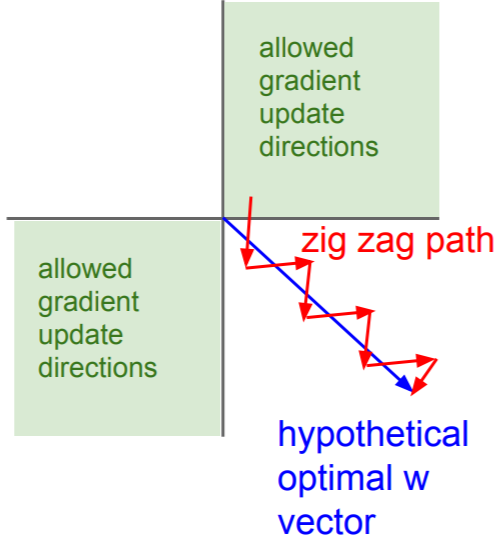
\includegraphics[keepaspectratio, scale=0.3]{pic/zigzag}
	\end{textblock*}

	\begin{itemize}
		\item Reminder: sigmoid
		\item Consider what happens when the input \newline to a neuron is always positive...
		\item What can we say about the gradients on w? \newline \textcolor{red}{Always all positive or all negative}
		\begin{itemize}
			\item this is also why you want zero-mean data!
		\end{itemize}
	\end{itemize}
	
\end{frame}

\begin{frame}{Why normalize the input?}
	
	\begin{textblock*}{5cm}(9cm,1.5cm) % {block width} (coords)
		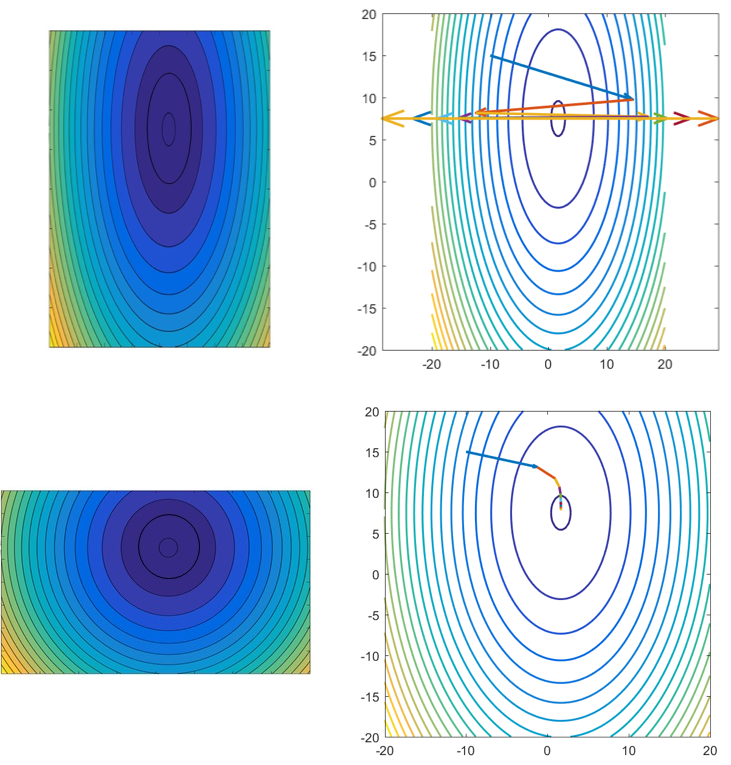
\includegraphics[keepaspectratio, scale=0.25]{pic/poorcond}
	\end{textblock*}
	
	\begin{itemize}
		\item Very different range of input features
		\item i.e. poor conditioning
		\item causes noisy movement of gradient
	\end{itemize}
	\vspace{1.5cm}
	\begin{itemize}
		\item Normalized data:
		\begin{itemize}
			\item improves loss landscape \newline (alleviate poor conditioning)
			\item faster optimization (training)
		\end{itemize}
	\end{itemize}
	
\end{frame}

\begin{frame}
	\begin{figure}[htpb]
		\begin{center}
			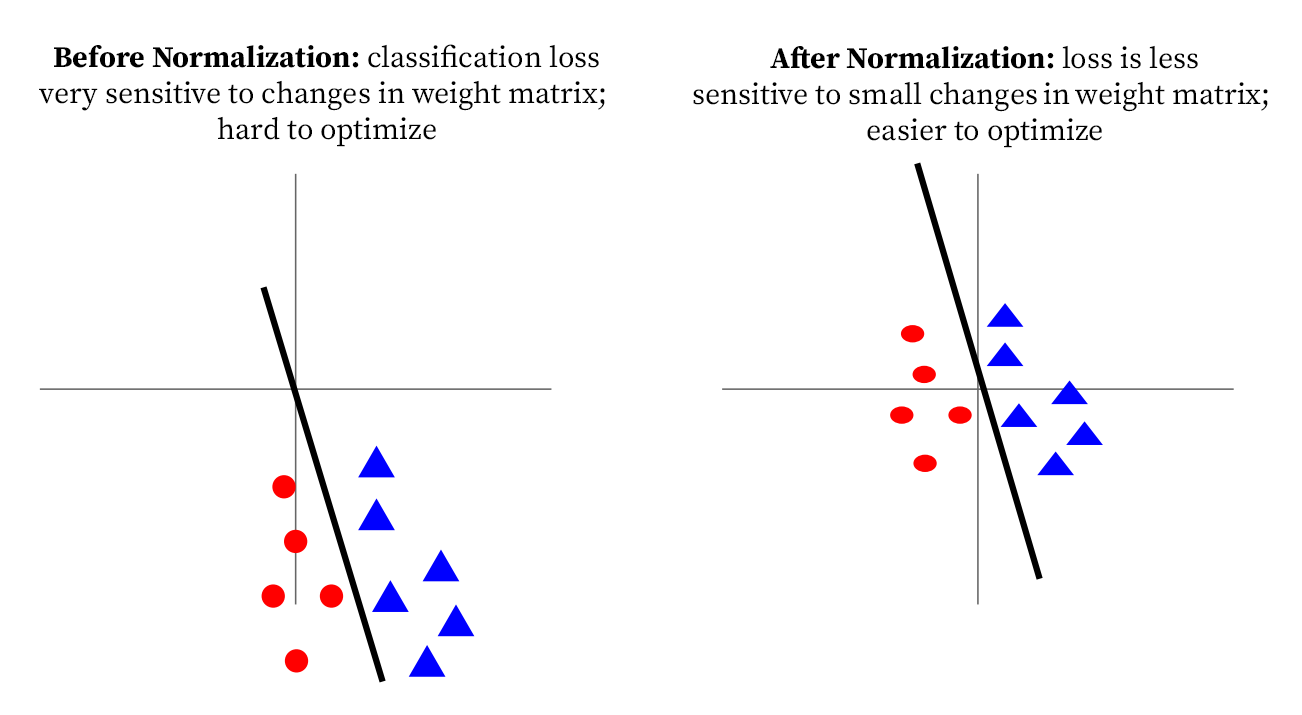
\includegraphics[keepaspectratio, scale=0.3]{pic/normaliz2}
		\end{center}
	\end{figure}	
\end{frame}


\begin{frame}{Not common to normalize variance, to do PCA or whitening}
	\begin{figure}[htpb]
		\begin{center}
			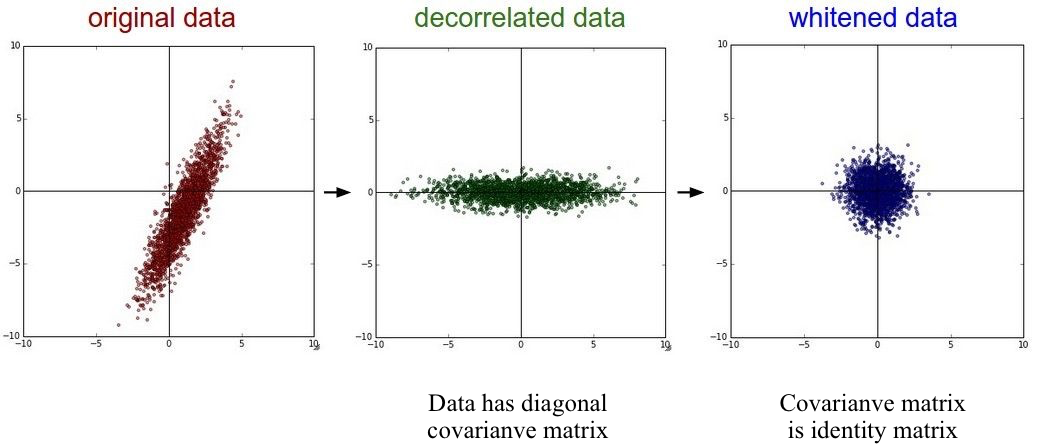
\includegraphics[keepaspectratio, scale=0.35]{pic/whiten}
		\end{center}
	\end{figure}	
\end{frame}

\section{Data Augmentation}

\begin{frame}{Motivation}
	\begin{textblock*}{5cm}(7.2cm,3.7cm) % {block width} (coords)
		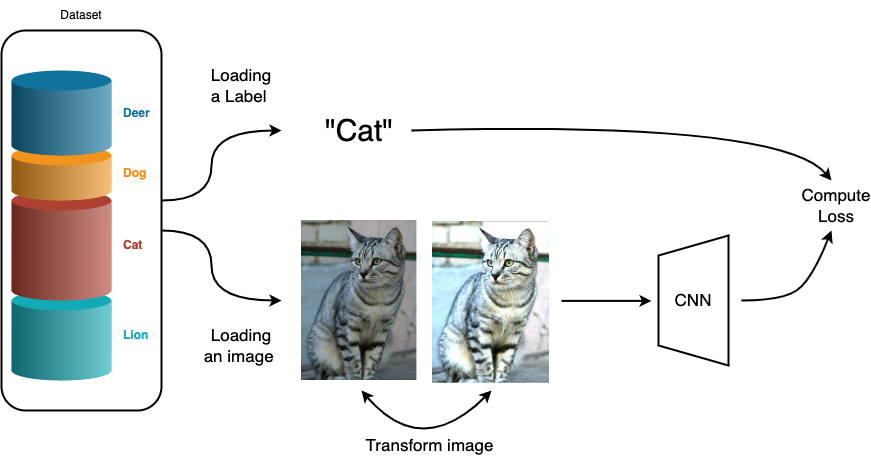
\includegraphics[keepaspectratio, scale=0.28]{pic/cnnaug}
	\end{textblock*}
	
	\begin{itemize}
		\item Getting more training data can be expensive
		\item But, sometimes we can generate more training examples from the datasets
		\item Transform each input data example in such a way that the label stays the same
		\item Benefits:
		\begin{itemize}
			\item Reduces Overfitting 
			\item Improves generalization
			\item Acts as a regularization
		\end{itemize}
		\item Examples of data augmentations
		\begin{itemize}
			\item Translation
			\item Rotation
			\item Stretching
			\item Shearing
			\item Lens distortions, … (go crazy)
		\end{itemize}
	\end{itemize}
\end{frame}

\begin{frame}{Examples of data augmentations}
	\begin{figure}[htpb]
		\begin{center}
			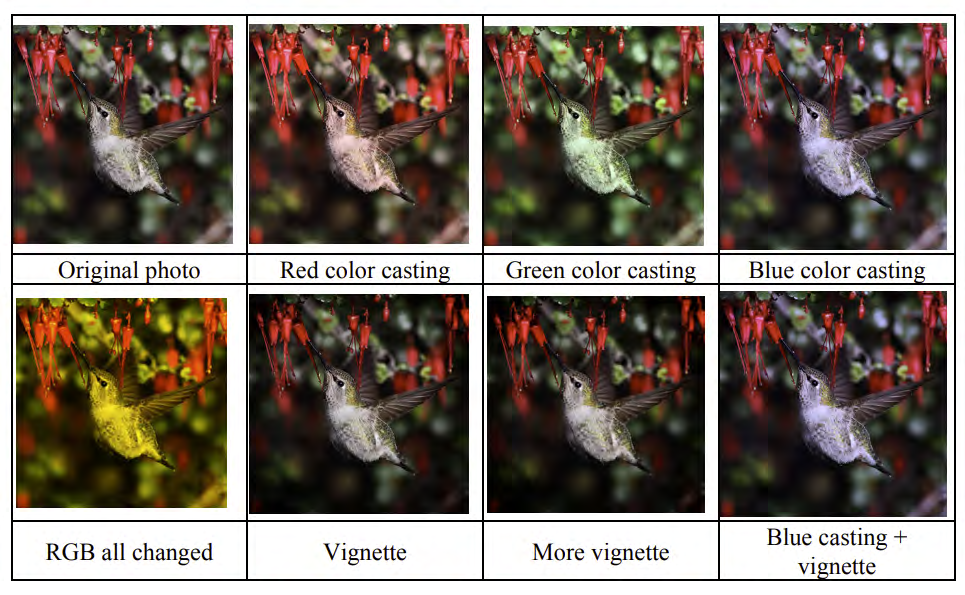
\includegraphics[keepaspectratio, scale=0.29]{pic/augm}
			\caption*{\scriptsize{Wu, R., et al. ``Deep image: Scaling up image recognition'' (2015)}}
		\end{center}
	\end{figure}
\end{frame}

\begin{frame}{Augmentations in action}
	\begin{textblock*}{7cm}(8.5cm,2.2cm) % {block width} (coords)
		\begin{figure}
			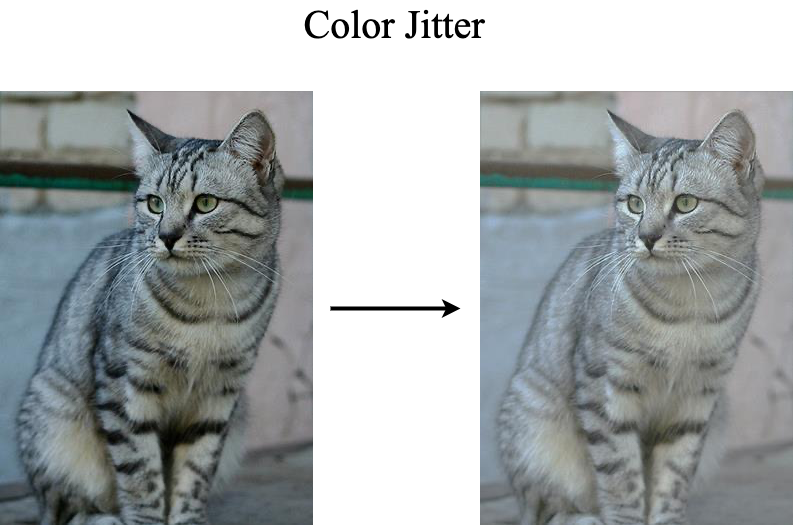
\includegraphics[keepaspectratio, scale=0.24]{pic/jitter}
			\caption*{\tiny{\href{https://www.flickr.com/photos/malfet/1428198050}{\color{blue} This image} by \href{https://www.flickr.com/photos/malfet/}{\color{blue} Nikita} is licensed under \href{https://creativecommons.org/licenses/by/2.0/}{\color{blue} CC-BY 2.0}}}
		\end{figure}

	\end{textblock*}
	
	\begin{itemize}
		\item Simple
		\begin{itemize}
			\item Randomize contrast and brightness
		\end{itemize}
		\item Complex
		\begin{enumerate}
			\item Apply PCA to all [R, G, B] pixels \newline in training set
			\item Sample a “color offset” along principal \newline component directions
			\item Add offset to all pixels of a training \newline image
			\newline \small{(As seen in AlexNet, ResNet, etc)}
		\end{enumerate}
	\end{itemize}
\end{frame}

\begin{frame}{Augmentations in action}
	\begin{textblock*}{5cm}(10cm,2.2cm) % {block width} (coords)
		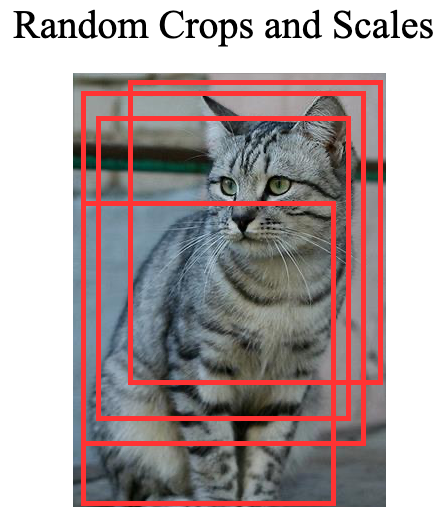
\includegraphics[keepaspectratio, scale=0.28]{pic/crop}
	\end{textblock*}

	\begin{itemize}
	\item \textbf{Training:} sample random crops / scales \newline ResNet:
		\begin{enumerate}
				\item Pick random L in range [256, 480]
				\item Resize training image, short side = L
				\item Sample random 224 x 224 patch
		\end{enumerate}
		
	\item \textbf{Testing:} average a fixed set of crops \newline ResNet:
		\begin{enumerate}
			\item Resize image at 5 scales: {224, 256, 384, 480, 640}
			\item For each size, use 10 224 x 224 crops: \newline 4 corners + center, + flips
		\end{enumerate}				
	\end{itemize}
\end{frame}


\begin{frame}{Augmentations in action}
	\begin{textblock*}{5cm}(10cm,1.5cm) % {block width} (coords)
		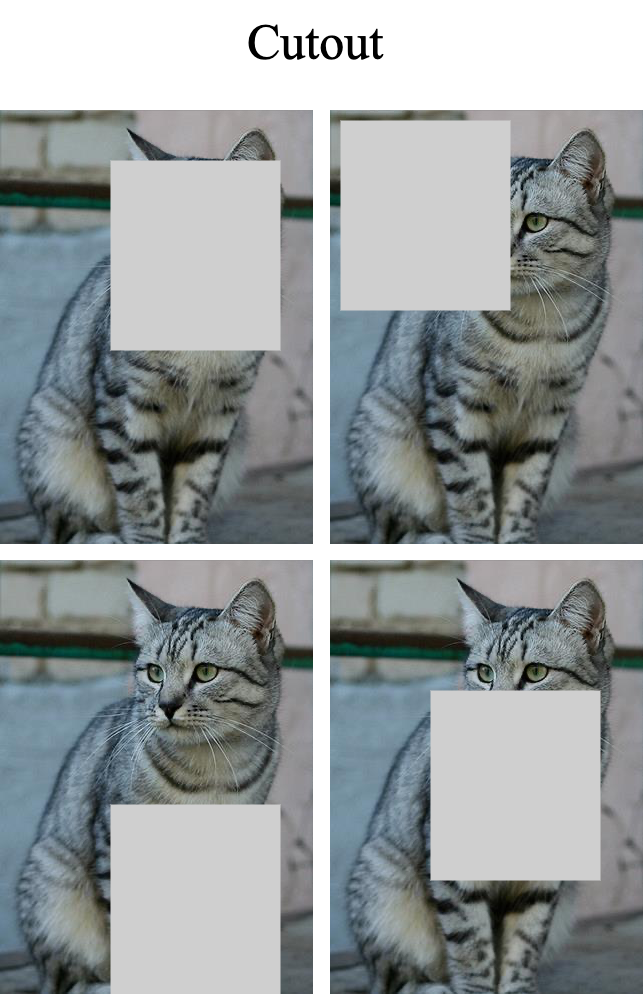
\includegraphics[keepaspectratio, scale=0.18]{pic/cutout}
	\end{textblock*}

	\begin{itemize}
		\item \textbf{Training:} Set random image regions to zero 
		\item \textbf{Testing:} Use full image
		\item Works very well for small datasets like CIFAR, less \newline common for large datasets like ImageNet
	\end{itemize}

	\begin{textblock*}{10cm}(1.5cm,8.2cm) % {block width} (coords)
		\tiny{DeVries and Taylor, ``Improved Regularization of Convolutional
		Neural Networks with Cutout'', arXiv 2017}
	\end{textblock*}	

	
\end{frame}


\section{Transfer Learning}

\begin{frame}{Motivation}
	\begin{figure}[htpb]
		\begin{center}
			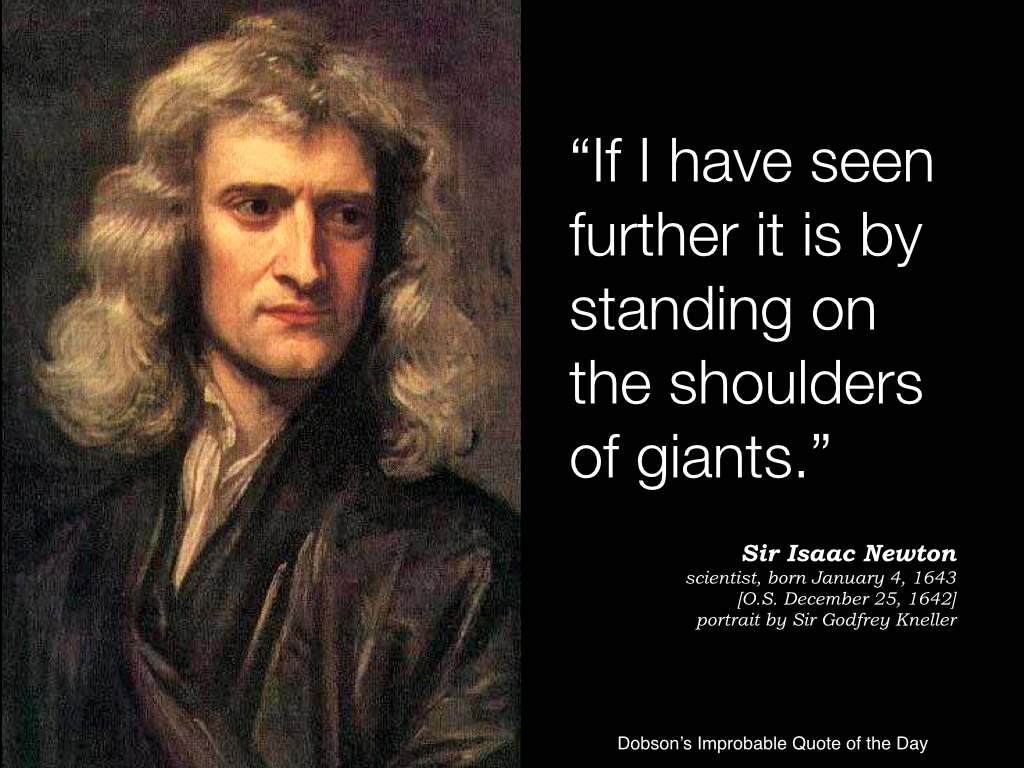
\includegraphics[keepaspectratio, scale=0.25]{pic/giant}
		\end{center}
	\end{figure}
\end{frame}

\begin{frame}{Motivation}
	\begin{itemize}
		\item You need a lot of a data if you want to train/use CNNs
		\item Suppose you want to build an app to recognize flowers…
	\end{itemize}
	\begin{figure}[htpb]
		\begin{center}
			\includegraphics[keepaspectratio, scale=0.25]{pic/TL_motiv}
			\caption*{https://www.robots.ox.ac.uk/~vgg/data/flowers/102}
		\end{center}
	\end{figure}
\end{frame}

\begin{frame}{Transfer learning}
	\begin{itemize}
		\item However, by transfer learning you can use the learned features for a task (using a large amount of data) in another related task (for which you don’t have enough data)
		\item \textbf{what should we train?}
		\item Option 1: Train only classification layer, freeze backbone

		\setbeamertemplate{itemize subitem}{$\rightarrow$}
		\begin{itemize}
			\item sometimes referred to as the “linear evaluation protocol”
			\item Fast \& simple
		\end{itemize}
		\item Option 2: Train classification layer, fine-tune backbone at the same time

		\setbeamertemplate{itemize subitem}{$\rightarrow$}
		\begin{itemize}
			\item Slower, but can adapt feature extraction to dataset statistics
		\end{itemize}
	\end{itemize}
\end{frame}

\begin{frame}{Transfer learning: The idea}
	\vspace{-1em}
	\begin{figure}[htpb]
		\begin{center}
			\includegraphics[keepaspectratio, scale=0.23]{pic/TL_alexnet}
		\end{center}
	\end{figure}
\end{frame}

\begin{frame}{Transfer Learning with CNNs}
	\begin{figure}[htpb]
		\begin{center}
			\includegraphics[keepaspectratio, scale=0.25]{pic/TL_cnn}
			\caption*{\scriptsize Donahue et al, “DeCAF: A Deep Convolutional Activation Feature for Generic Visual Recognition”, ICML 2014 \newline Razavian et al, “CNN Features Off-the-Shelf: An Astounding Baseline for Recognition”, CVPR Workshops 2014}
		\end{center}
	\end{figure}
\end{frame}

\begin{frame}{Transfer Learning with CNNs}
	\begin{figure}[htpb]
		\begin{center}
			\includegraphics[keepaspectratio, scale=0.25]{pic/TL_cnn2}
		\end{center}
	\end{figure}
\end{frame}

\begin{frame}{Transfer Learning with CNNs}
	\begin{figure}[htpb]
		\begin{center}
			\includegraphics[keepaspectratio, scale=0.25]{pic/TL_cnn3}
		\end{center}
	\end{figure}
\end{frame}

\begin{frame}{Transfer learning with CNNs}
	\begin{figure}[htpb]
		\begin{center}
			\includegraphics[keepaspectratio, scale=0.25]{pic/TL_idea}
		\end{center}
	\end{figure}
\end{frame}

\begin{frame}{Transfer learning: Domain Change}
	\begin{figure}[htpb]
		\begin{center}
			\includegraphics[keepaspectratio, scale=0.25]{pic/TL_domain_change}
		\end{center}
	\end{figure}
\end{frame}

\begin{frame}{Example: semantic segmentation}
	\begin{figure}[htpb]
		\begin{center}
			\includegraphics[keepaspectratio, scale=0.25]{pic/sem}
			\caption*{\scriptsize Long, Shelhamer, Darrell, CVPR 2015}
		\end{center}
	\end{figure}
\end{frame}

\begin{frame}{Example: Single-stage object detectors: SSD, YOLO, …}
	\begin{figure}[htpb]
		\begin{center}
			\includegraphics[keepaspectratio, scale=0.25]{pic/ssd}
			\caption*{\scriptsize Liu et al., ECCV 2016 | Redmon et al., CVPR 2016 | Lin et al., CVPR 2017}
		\end{center}
	\end{figure}
\end{frame}

\begin{frame}{Transfer learning with CNNs is pervasive…}
	\begin{figure}[htpb]
		\begin{center}
			\includegraphics[keepaspectratio, scale=0.25]{pic/TL_examples}
		\end{center}
	\end{figure}
\end{frame}

\begin{frame}{Transfer learning with CNNs is pervasive…}
	\begin{figure}[htpb]
		\begin{center}
			\includegraphics[keepaspectratio, scale=0.25]{pic/TL_examples2}
			\caption*{\scriptsize Girshick, “Fast R-CNN”, ICCV 2015 Figure copyright Ross Girshick, 2015. Reproduced with permission., Karpathy and Fei-Fei, “Deep Visual-Semantic Alignments for Generating Image Descriptions”, CVPR 2015 Figure copyright IEEE, 2015. Reproduced for educational purposes.}
		\end{center}
	\end{figure}
\end{frame}

\begin{frame}{Architecture matters}
	\begin{figure}[htpb]
		\begin{center}
			\includegraphics[keepaspectratio, scale=0.25]{pic/od_mscoco}
			\captionsetup{justification=centering}
			\caption*{\scriptsize Girshick, “The Generalized R-CNN Framework for Object Detection”, ICCV 2017}
		\end{center}
	\end{figure}
\end{frame}

\begin{frame}{Transfer Learning might not always be necessary!}
	\begin{itemize}
		\item Training from scratch can work just \newline as well as training from a pretrained
		\newline ImageNet model for object detection
		\item But it takes 2-3x as long to train.
		\item They also find that collecting more \newline data is better than finetuning on a 
		\newline related task
	\end{itemize}
	\begin{textblock*}{5cm}(9cm,1.3cm) % {block width} (coords)
		\begin{figure}
			\includegraphics[keepaspectratio, scale=0.28]{pic/rethinking_imagenet}
			\caption*{\scriptsize He et al, “Rethinking ImageNet Pre-training”, ICCV 2019 Figure copyright Kaiming He, 2019. Reproduced with permission.}
		\end{figure}
	\end{textblock*}
\end{frame}

\begin{frame}{What is being transferred?}
	\begin{figure}[htpb]
		\begin{center}
			\includegraphics[keepaspectratio, scale=0.15]{pic/what_TL}
			\caption*{\scriptsize Neyshabour et al, What is being transferred in transfer learning?, NeurIPS 2020}
		\end{center}
	\end{figure}
\end{frame}

\begin{frame}{Performance barrier between different solutions}
	\begin{itemize}
		\item There is no performance barriers between finetune models
		\item Finetune models reside in the same basin
		\item RandInits end up in a different basin, even for the same random seed
	\end{itemize}
	
	\begin{figure}
		\includegraphics[keepaspectratio, scale=0.22]{pic/what_TL2}
		\vspace{-1em}
		\caption*{\scriptsize He et al, “Rethinking ImageNet Pre-training”, ICCV 2019 Figure: Kaiming He, 2019}
	\end{figure}
\end{frame}

\begin{frame}{Takehome message}
	\begin{itemize}
		\item Have some dataset of interest but it has $< \texttildelow$ 1M images?
		\begin{enumerate}
			\item Find a very large dataset that has similar data, train a big ConvNet there
			\item Transfer learn to your dataset
		\end{enumerate}
		\item Deep learning frameworks provide a "Model Zoo" of pretrained models so you dont need to train your own
		\begin{itemize}
			\item \textbf{Pytorch:} \href{https://github.com/pytorch/vision}{\color{blue} https://github.com/pytorch/vision}
			\item \textbf{TensorFlow:} \href{https://github.com/tensorflow/models}{\color{blue} https://github.com/tensorflow/models}
		\end{itemize}

	\end{itemize}
\end{frame}

\section{References}

\begin{frame}[allowframebreaks]
	\bibliography{ref}
	\bibliographystyle{ieeetr}
	\nocite{*} % used here because no citation happens in slides
	% if there are too many try use:
	% \tiny\bibliographystyle{alpha}
\end{frame}


\begin{frame}
	\begin{center}
		{\Huge Any Questions?}
	\end{center}
\end{frame}

\end{document}